\documentclass[a4paper,11pt]{article}

\usepackage{graphicx}
\usepackage{hyperref}
\usepackage[a4paper, left=2.5cm, right=2.5cm, top=2.5cm, bottom=2.5cm]{geometry}
\usepackage{times}
\usepackage{amsmath}
\usepackage{booktabs} 
\usepackage{longtable}
\usepackage{tocloft}
\usepackage{fancyhdr}
\usepackage{float}
\usepackage{pgf,pgffor}
\usepackage{tcolorbox}


\renewcommand{\cftsecfont}{\large}
\renewcommand{\cftsubsecfont}{\normalsize}
\renewcommand{\cftsubsubsecfont}{\small}

\hypersetup{
    colorlinks=true,
    linkcolor= black,
    filecolor=magenta,      
    urlcolor=cyan,
    citecolor=blue,
}

\renewcommand{\contentsname}{Table des Matières}

\pagestyle{fancy}
\fancyhead{}
\setlength{\footskip}{33pt}
\fancyfoot[C]{
\includegraphics[width=1cm]{img/logo.jpg}}
\fancyfoot[L]{\textit{MECEN}}
\fancyfoot[R]{\thepage}



\usepackage{Sweave}
\begin{document}
\Sconcordance{concordance:dosfin.tex:dosfin.Rnw:1 39 1 1 0 3 1 1 52 1 18 1 12 102 1 1 %
4 32 0 1 2 8 1 1 15 1 2 46 1 1 27 32 0 1 2 11 1 1 8 1 2 12 1 2 2 8 1 1 %
2 11 0 1 2 19 1 1 4 1 1 1 6 13 0 1 2 7 1 1 12 20 0 1 2 8 1 1 6 1 2 12 1 %
2 2 25 1 1 2 4 0 1 2 3 1 1 3 5 0 1 2 6 1 1 13 15 0 1 2 71 1 1 6 2 1 1 8 %
1 2 8 1 1 8 1 2 1 4 15 0 1 2 11 1 1 6 1 1 1 2 18 0 1 2 7 1 1 17 1 3 8 1 %
1 10 1 2 14 1 1 4 5 1 1 2 18 0 1 2 6 1 1 17 1 3 6 1 1 10 1 2 18 1 1 5 3 %
1 2 2 13 1 1 2 18 0 1 2 6 1 1 17 1 3 6 1 1 10 1 2 18 1 1 5 3 1 2 2 12 1 %
1 2 18 0 1 2 6 1 1 17 1 3 6 1 1 10 1 2 18 1 1 5 3 1 2 2 13 1 1 2 18 0 1 %
2 6 1 1 17 1 3 6 1 1 10 1 2 22 1 1 5 3 1 2 2 14 1 1 2 18 0 1 2 6 1 1 17 %
1 3 6 1 1 10 1 2 26 1 1 5 3 1 2 2 16 1 1 2 18 0 1 2 6 1 1 17 1 3 6 1 1 %
10 1 2 7 1 1 5 1 2 6 1 1 16 1 2 29 1 1 5 3 1 1 14 1 2 14 1 1 2 18 0 1 2 %
6 1 1 17 1 3 6 1 1 10 1 2 7 1 1 15 1 2 26 1 1 5 3 1 2 2 37 1 1 17 1 3 6 %
1 1 10 1 2 7 1 1 7 1 1 1 3 1 2 16 1 1 22 1 2 17 1}








\begin{titlepage}
    \begin{center}
    
        \vspace{2cm}
        \Huge
        \textbf{Cancer prediction}
            
        \vspace{1cm}
        \LARGE
        Prédiction du risque d'avoir un cancer du poumon
            
        \vspace{3cm}
            
        Projet de recherche réalisé dans le cadre du master 1 MECEN
            
        \vspace{7cm}
            
        
\includegraphics[width=0.4\textwidth]{img/logo.jpg}

        \vspace{2cm}

        \Large
        Université de Tours \\

        Par Alexis VINCENT et Jawad GRIB

        2024-2025
            
    \end{center}
    
\end{titlepage}

\begin{center}
    \tableofcontents
\end{center}

\newpage

\section{Présentation des données}

L'étude porte sur un échantillon de \textbf{1000 individus}. Chaque individu est décrit par \textbf{22 variables explicatives}, toutes ordinales discrètes, ainsi qu'une variable dépendante \texttt{Level} représentant le \textit{risque de cancer du poumon}, catégorisé en trois modalités : \textbf{Low}, \textbf{Medium} et \textbf{High}.

Parmi les variables explicatives, seule la variable \texttt{Age} est numérique. Toutes les autres variables sont codées sous forme de niveaux, avec des échelles allant de \textbf{0 à 7}, \textbf{0 à 8} ou \textbf{0 à 9}, selon les cas. Ces échelles représentent des niveaux d'exposition, de sévérité ou d'habitudes, selon les thématiques abordées.

\vspace{1em}

\begin{table}[H]
\centering
\small
\renewcommand{\arraystretch}{1.2}
\begin{tabular}{|l|p{10cm}|}
\hline
\textbf{Nom de la variable} & \textbf{Description} \\
\hline
\texttt{Age} & Âge du patient (numérique). \\
\texttt{Air Pollution} & Niveau d'exposition à la pollution de l'air (catégorielle ordinale). \\
\texttt{Alcohol use} & Niveau de consommation d'alcool (catégorielle ordinale). \\
\texttt{Dust Allergy} & Niveau d'allergie à la poussière (catégorielle ordinale). \\
\texttt{Occupational Hazards} & Niveau d'exposition à des risques professionnels (catégorielle ordinale). \\
\texttt{Genetic Risk} & Niveau de risque génétique (catégorielle ordinale). \\
\texttt{Chronic Lung Disease} & Niveau de gravité d'une maladie pulmonaire chronique (catégorielle ordinale). \\
\texttt{Balanced Diet} & Niveau d'équilibre alimentaire (catégorielle ordinale). \\
\texttt{Obesity} & Niveau d'obésité (catégorielle ordinale). \\
\texttt{Smoking} & Niveau de tabagisme actif (catégorielle ordinale). \\
\texttt{Passive Smoker} & Niveau d'exposition au tabagisme passif (catégorielle ordinale). \\
\texttt{Chest Pain} & Intensité des douleurs thoraciques (catégorielle ordinale). \\
\texttt{Coughing of Blood} & Sévérité des épisodes d'hémoptysie (catégorielle ordinale). \\
\texttt{Fatigue} & Niveau de fatigue (catégorielle ordinale). \\
\texttt{Weight Loss} & Niveau de perte de poids (catégorielle ordinale). \\
\texttt{Shortness of Breath} & Niveau de dyspnée (catégorielle ordinale). \\
\texttt{Wheezing} & Intensité des sifflements respiratoires (catégorielle ordinale). \\
\texttt{Swallowing Difficulty} & Niveau de difficulté à avaler (catégorielle ordinale). \\
\texttt{Clubbing of Finger Nails} & Niveau d'hippocratisme digital (catégorielle ordinale). \\
\texttt{Frequent Cold} & Fréquence des rhumes (catégorielle ordinale). \\
\texttt{Dry Cough} & Niveau de toux sèche (catégorielle ordinale). \\
\texttt{Snoring} & Fréquence du ronflement (catégorielle ordinale). \\
\hline
\end{tabular}
\caption{Description des variables explicatives du jeu de données.}
\end{table}


\vspace{1em}

La variable cible, \texttt{Level}, représente la \textbf{probabilité qu'un individu soit atteint d’un cancer du poumon}, codée en trois classes : 

\begin{itemize}
  \item \textbf{Low} : Faible risque
  \item \textbf{Medium} : Risque modéré
  \item \textbf{High} : Risque élevé
\end{itemize}

\newpage

\section{Etudes statistique}

\subsection{Distribution des données}


\begin{center}
% latex table generated in R 4.4.3 by xtable 1.8-4 package
% Sun Apr 20 03:36:57 2025
\begin{table}[ht]
\centering
\begin{tabular}{rllrr}
  \hline
 & skim\_type & skim\_variable & numeric.mean & numeric.sd \\ 
  \hline
1 & numeric & Age & 37.17 & 12.01 \\ 
  2 & numeric & Air.Pollution & 3.84 & 2.03 \\ 
  3 & numeric & Alcohol.use & 4.56 & 2.62 \\ 
  4 & numeric & Dust.Allergy & 5.16 & 1.98 \\ 
  5 & numeric & OccuPational.Hazards & 4.84 & 2.11 \\ 
  6 & numeric & Genetic.Risk & 4.58 & 2.13 \\ 
  7 & numeric & chronic.Lung.Disease & 4.38 & 1.85 \\ 
  8 & numeric & Balanced.Diet & 4.49 & 2.14 \\ 
  9 & numeric & Obesity & 4.46 & 2.12 \\ 
  10 & numeric & Smoking & 3.95 & 2.50 \\ 
  11 & numeric & Passive.Smoker & 4.20 & 2.31 \\ 
  12 & numeric & Chest.Pain & 4.44 & 2.28 \\ 
  13 & numeric & Coughing.of.Blood & 4.86 & 2.43 \\ 
  14 & numeric & Fatigue & 3.86 & 2.24 \\ 
  15 & numeric & Weight.Loss & 3.85 & 2.21 \\ 
  16 & numeric & Shortness.of.Breath & 4.24 & 2.29 \\ 
  17 & numeric & Wheezing & 3.78 & 2.04 \\ 
  18 & numeric & Swallowing.Difficulty & 3.75 & 2.27 \\ 
  19 & numeric & Clubbing.of.Finger.Nails & 3.92 & 2.39 \\ 
  20 & numeric & Frequent.Cold & 3.54 & 1.83 \\ 
  21 & numeric & Dry.Cough & 3.85 & 2.04 \\ 
  22 & numeric & Snoring & 2.93 & 1.47 \\ 
   \hline
\end{tabular}
\caption{Destributions des variables} 
\end{table}
\end{center}

On note ici que les variables, à l'exception de l'âge, semblent avoir des moyennes très proches et des écarts-types avoisinant 2. Ainsi, il n'y aura pas d'effet d'échelle conséquent sur des modèles tels que \textit{LDA}, \textit{QDA} ou \textit{KNN}. Par conséquent, nous n'aurons pas besoin de centrer et réduire nos variables.


\subsection{Boxplot des variables en fonction du niveau de risque}

\begin{center}
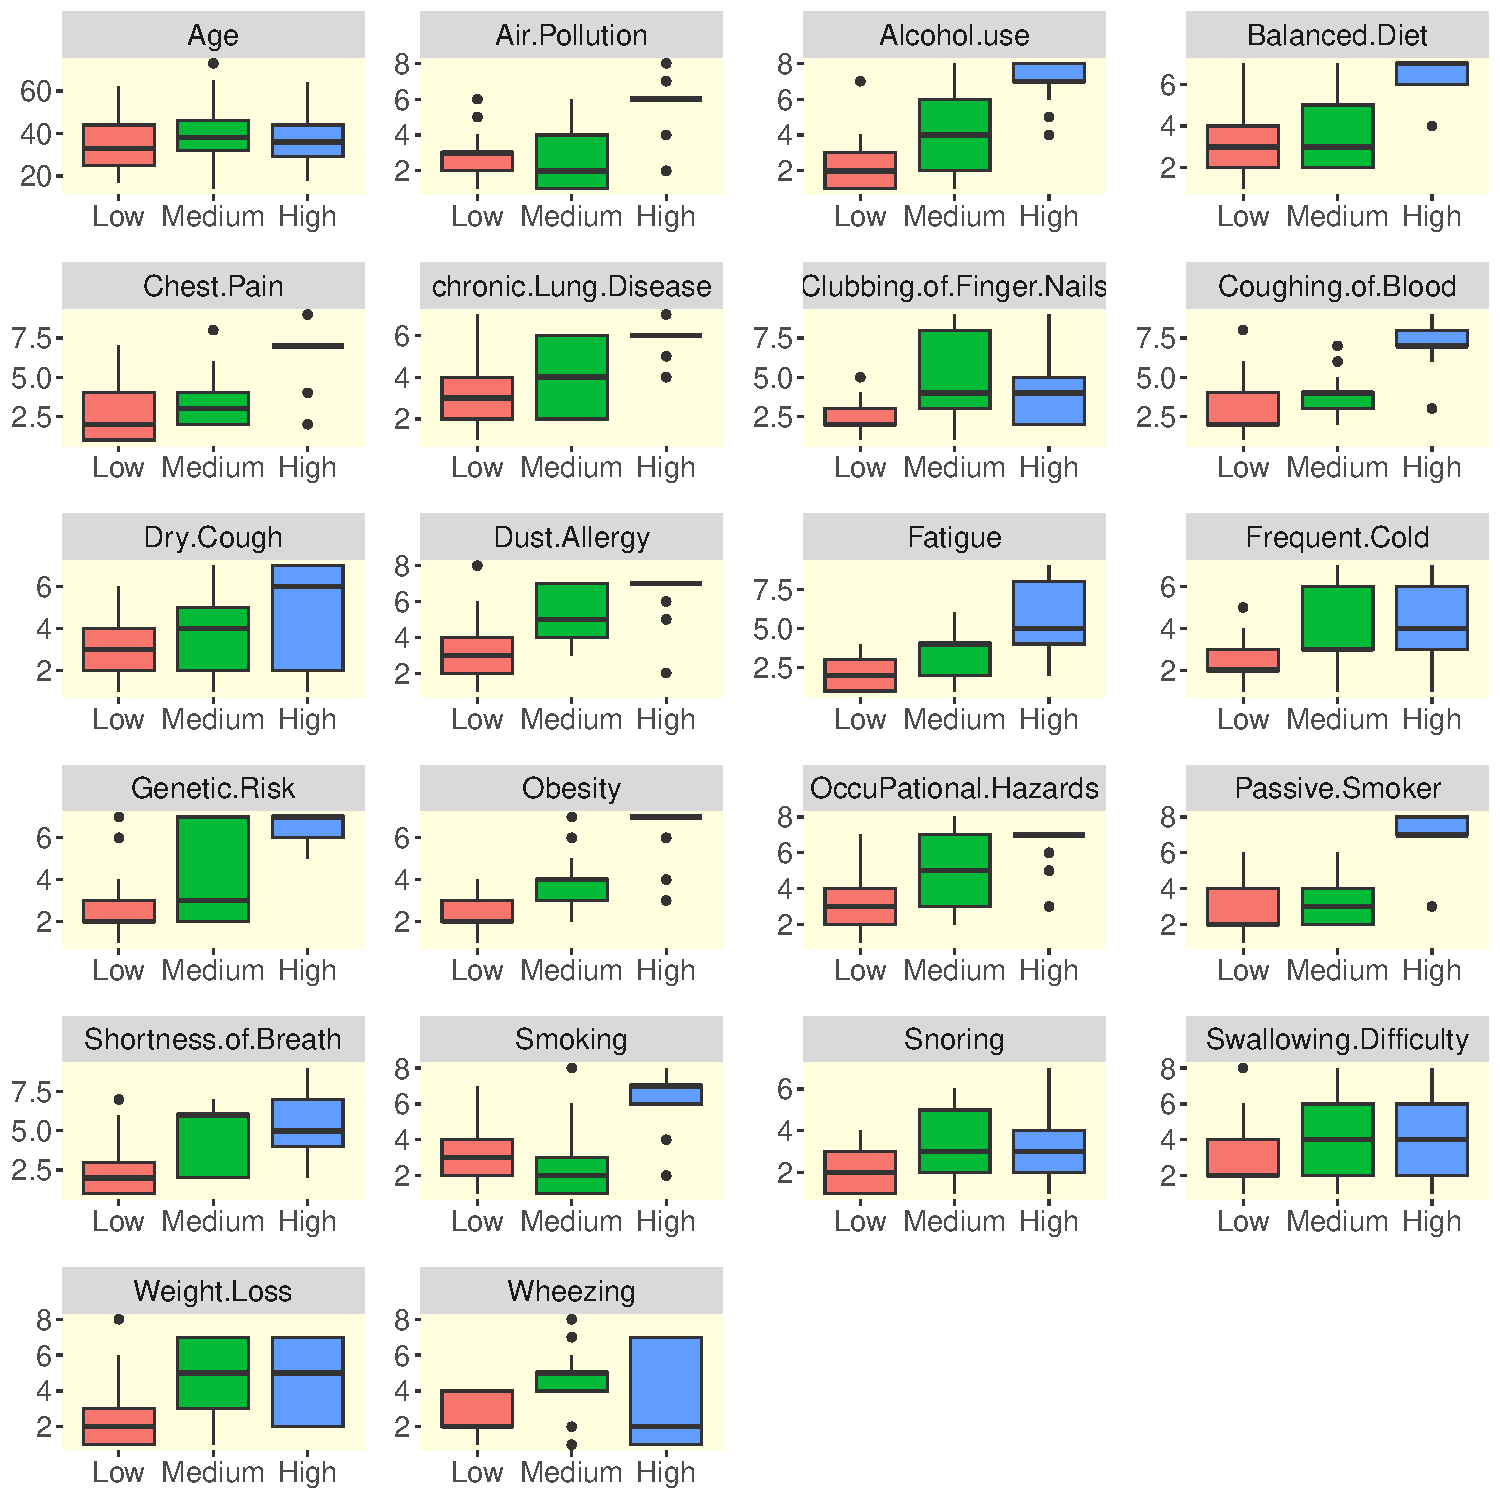
\includegraphics{dosfin-Boxplot}

\end{center}

Les boxplots mettent en évidence deux éléments principaux.\\
Tout d’abord, ils permettent d’identifier certaines variables potentiellement informatives : en effet, lorsqu’une variable présente des distributions nettement distinctes selon les classes de la variable cible (écart entre les boîtes, position des médianes), cela suggère qu’elle pourrait apporter beaucoup d'information à nos modèles.

\vspace{1em}

Par ailleurs, on observe la présence de nombreux \textit{outliers} dans plusieurs variables. Cette caractéristique pourrait affecter négativement les performances de certains modèles sensibles à la distribution des données, tels que la LDA, la QDA ou encore le KNN.

\vspace{1em}

Nous détaillerons plus loin dans cette étude la stratégie envisagée pour traiter ce problème.

\newpage

\subsection{Test ANOVA}

\subsubsection{Définition}

\begin{tcolorbox}[colback=gray!10, colframe=black, title=Test d'ANOVA à un facteur, fonttitle=\bfseries]
Afin de vérifier la significativité des variables explicatives par rapport à la variable à prédire, nous réalisons un \textbf{test d'ANOVA à un facteur}.

\bigskip

\textbf{Hypothèses du test :}
\begin{equation}
H_0 : \mu_1 = \mu_2 = \dots = \mu_k
\end{equation}
\begin{equation}
H_1 : \exists\, i \neq j \quad \text{tel que} \quad \mu_i \neq \mu_j
\end{equation}

\bigskip

\textbf{Interprétation :} \\
Même si nous disposons de plus de 100 observations, il est pertinent de confirmer statistiquement l’intérêt des variables. Le test d’ANOVA permet de déterminer si au moins un groupe présente une moyenne significativement différente.

\bigskip

\textbf{Règle de décision :} \\
Si la \textit{p-value} associée au test est inférieure au seuil de significativité \(\alpha = 0{,}05\), alors nous rejetons l’hypothèse nulle \(H_0\). Cela indique que la variable testée est potentiellement informative pour discriminer les classes de la variable cible.
\end{tcolorbox}

\subsubsection{Résultat}

\begin{center}
% latex table generated in R 4.4.3 by xtable 1.8-4 package
% Sun Apr 20 03:37:01 2025
\begin{table}[ht]
\centering
\begin{tabular}{rlrrr}
  \hline
 & Variable & Df & F\_value & p\_value \\ 
  \hline
1 & Obesity & 2.00 & 1190.54 & 0.00 \\ 
  2 & Coughing.of.Blood & 2.00 & 1037.56 & 0.00 \\ 
  3 & Passive.Smoker & 2.00 & 722.19 & 0.00 \\ 
  4 & Balanced.Diet & 2.00 & 689.94 & 0.00 \\ 
  5 & Dust.Allergy & 2.00 & 558.64 & 0.00 \\ 
  6 & Alcohol.use & 2.00 & 540.24 & 0.00 \\ 
  7 & Genetic.Risk & 2.00 & 488.98 & 0.00 \\ 
  8 & Air.Pollution & 2.00 & 466.79 & 0.00 \\ 
  9 & OccuPational.Hazards & 2.00 & 413.33 & 0.00 \\ 
  10 & Chest.Pain & 2.00 & 404.80 & 0.00 \\ 
  11 & Smoking & 2.00 & 369.48 & 0.00 \\ 
  12 & Fatigue & 2.00 & 328.93 & 0.00 \\ 
  13 & chronic.Lung.Disease & 2.00 & 316.05 & 0.00 \\ 
  14 & Shortness.of.Breath & 2.00 & 183.39 & 0.00 \\ 
  15 & Frequent.Cold & 2.00 & 127.07 & 0.00 \\ 
  16 & Wheezing & 2.00 & 111.40 & 0.00 \\ 
  17 & Clubbing.of.Finger.Nails & 2.00 & 107.65 & 0.00 \\ 
  18 & Weight.Loss & 2.00 & 97.65 & 0.00 \\ 
  19 & Dry.Cough & 2.00 & 81.85 & 0.00 \\ 
  20 & Snoring & 2.00 & 70.28 & 0.00 \\ 
  21 & Swallowing.Difficulty & 2.00 & 44.68 & 0.00 \\ 
  22 & Age & 2.00 & 5.75 & 0.00 \\ 
   \hline
\end{tabular}
\caption{Top 5 des variables selon la F-Value} 
\end{table}\end{center}

On observe que l'ensemble des variables rejette l'hypothèse nulle \(H_0\), ce qui signifie qu'elles sont toutes statistiquement significatives. Cela s’explique en partie par la taille de notre échantillon : avec 1000 individus, même de faibles différences entre groupes peuvent être considérées comme significatives.

Néanmoins, en croisant cette information avec les résultats issus des boxplots, on remarque que la variable \texttt{Age}, qui semblait visuellement la moins informative (distributions proches entre classes), est effectivement celle dont la \textit{F-value} est la plus faible.

Ainsi, la significativité globale des variables suggère que notre jeu de données est potentiellement bien structuré pour permettre une bonne séparation des classes à prédire à l’aide de modèles supervisés.

\subsection{Corrélation entre les variables}

\begin{center}

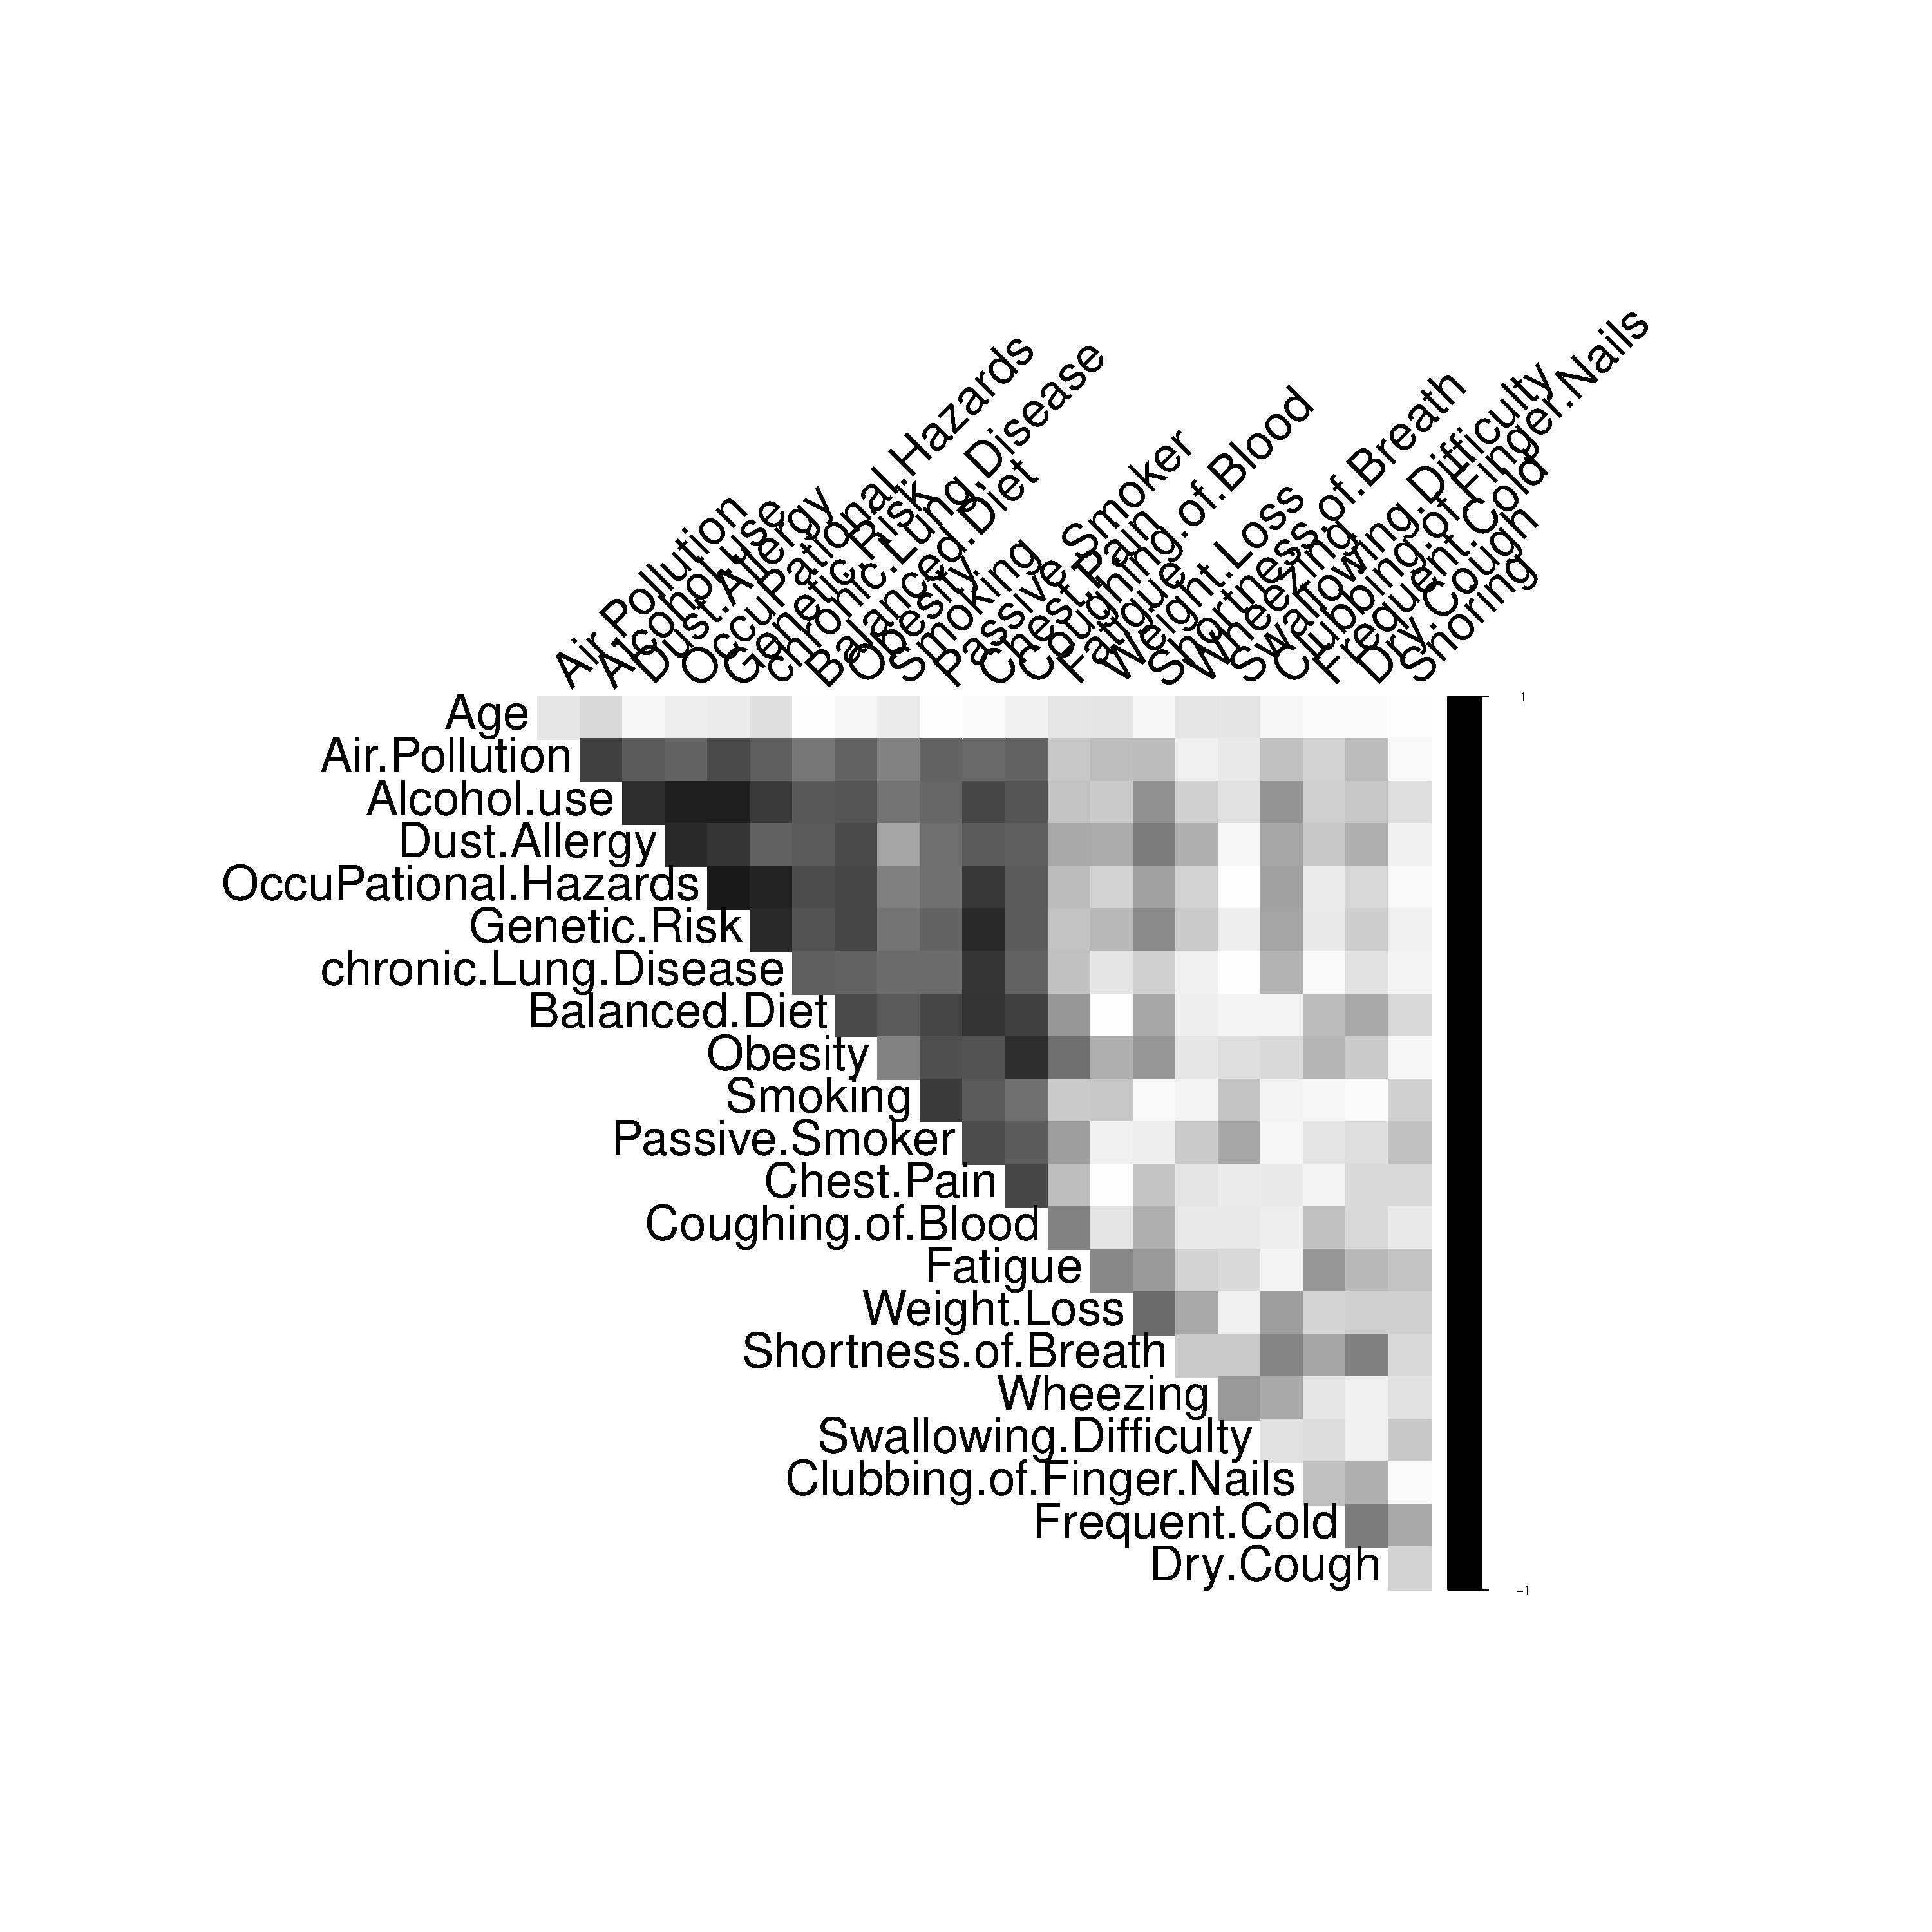
\includegraphics{dosfin-007}
\end{center}

  Ce graphique de corrélation met en évidence que de nombreuses variables semblent corrélées entre elles. Cette redondance d'information peut poser problème pour certains modèles sensibles à la multicolinéarité, comme la LDA, en faussant l’estimation des coefficients et en réduisant l’interprétabilité des résultats.

Pour remédier à ce problème, nous opterons pour la suppression de certaines variables fortement corrélées entre elles, en conservant uniquement celles qui apportent une information distincte ou jugée plus pertinente.


\newpage

\subsection{Valeurs manquantes}

\begin{center}

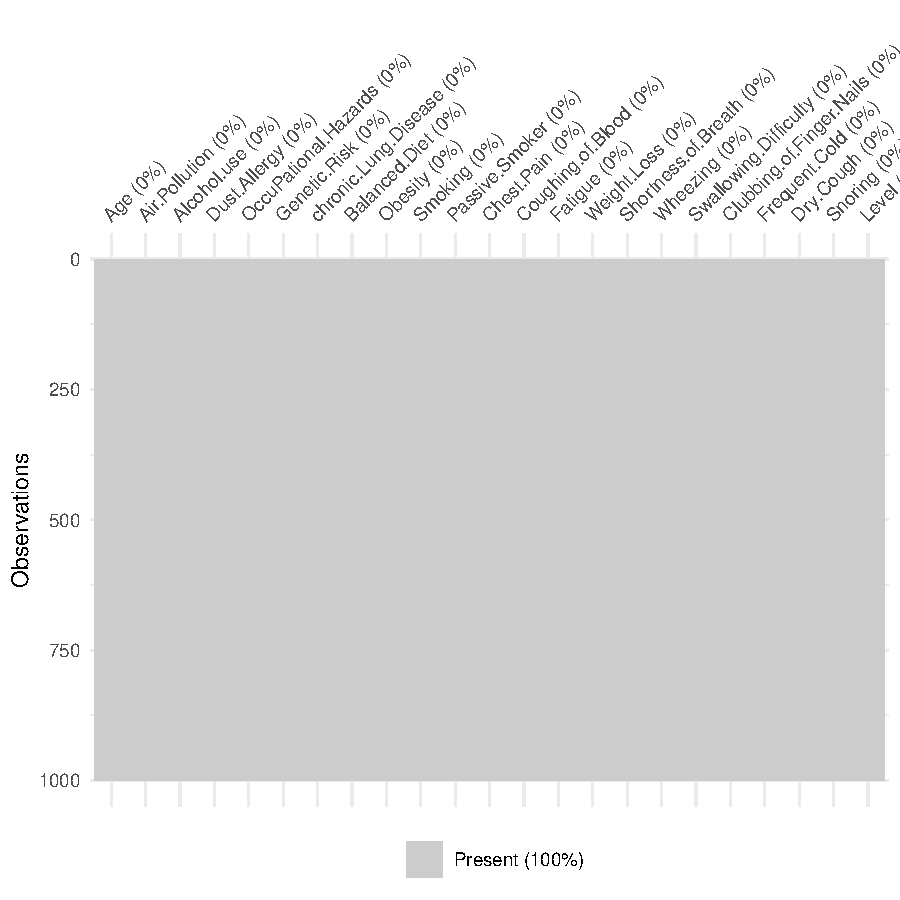
\includegraphics{dosfin-008}

\end{center}

On ne relève aucune valeur manquante dans le jeu de données. Cela constitue un point positif, car aucune stratégie d'imputation ou d'exclusion de données n’est nécessaire à cette étape. Nous pouvons donc poursuivre l’analyse sans ajustement préalable lié aux données absentes.

\subsection{Equilibre de la classe à prédire}

\begin{center}

% latex table generated in R 4.4.3 by xtable 1.8-4 package
% Sun Apr 20 03:37:01 2025
\begin{table}[ht]
\centering
\begin{tabular}{rrrr}
  \hline
 & Low & Medium & High \\ 
  \hline
1 & 303 & 332 & 365 \\ 
   \hline
\end{tabular}
\caption{Distribution du Risk d'avoir un cancer du poumons} 
\end{table}\end{center}

On constate que la classe à prédire est relativement équilibrée, ce qui est un bon signe pour la performance de nos modèles. En effet, une répartition équilibrée des classes permet d'éviter les biais qui peuvent survenir lorsqu'une classe est surreprésentée par rapport à une autre. Par conséquent, il n'est pas nécessaire de recourir à des techniques de prétraitement telles que SMOTE , qui génèrent artificiellement des exemples pour la classe minoritaire. En effet, si une classe est trop minoritaire, le modèle pourrait rencontrer des difficultés à prédire cette classe de manière fiable, au détriment des autres classes.


\newpage

\section{Analyse à composante principale}


\begin{itemize}
  \item Nous allons réaliser une ACP sur notre jeu de données afin d’observer les relations entre les variables.
  \item Ensuite, nous analyserons la projection des individus dans l’espace des composantes principales.
  \item L’objectif est de déterminer si les différentes classes sont bien séparées en fonction des caractéristiques propres à chaque individu.
\end{itemize}

\subsection{Etudes de l'inertie}

Nous allons ici identifier les plans qui capturent le plus d’inertie, afin de baser notre étude sur celui ou ceux qui contiennent le plus d'informations.


\begin{center}
% latex table generated in R 4.4.3 by xtable 1.8-4 package
% Sun Apr 20 03:37:01 2025
\begin{table}[ht]
\centering
\begin{tabular}{rrrrrr}
  \hline
 & F1 & F2 & F3 & F4 & F5 \\ 
  \hline
Valeur propre & 9.00 & 2.70 & 2.00 & 1.50 & 1.30 \\ 
  Variance & 41.10 & 12.30 & 9.20 & 6.90 & 5.70 \\ 
  Pourcentage de variance & 41.10 & 53.40 & 62.50 & 69.40 & 75.20 \\ 
   \hline
\end{tabular}
\caption{Tableau des inerties} 
\end{table}\end{center}

Pour cette étude, nous nous concentrerons sur le plan 1–2, qui contient 53.4\% de l’information du jeu de données, ainsi que sur le plan 2–3. Les autres axes, ayant des valeurs propres proches de 1, sont considérés comme négligeables pour notre analyse.

\subsection{Etudes des variables}

Voici les caractéristiques des variables:

% latex table generated in R 4.4.3 by xtable 1.8-4 package
% Sun Apr 20 03:37:01 2025
\begin{table}[ht]
\centering
\begin{tabular}{rrrrr}
  \hline
 & Coord\_F1 & Coord\_F2 & Contrib\_12 & Cos2\_12 \\ 
  \hline
Shortness.of.Breath & 0.47 & 0.71 & 21.03 & 0.72 \\ 
  Weight.Loss & 0.27 & 0.70 & 19.10 & 0.56 \\ 
  Smoking & 0.64 & -0.54 & 15.25 & 0.70 \\ 
  Clubbing.of.Finger.Nails & 0.30 & 0.61 & 15.02 & 0.47 \\ 
  Chest.Pain & 0.85 & -0.30 & 11.30 & 0.81 \\ 
  Passive.Smoker & 0.76 & -0.36 & 11.20 & 0.71 \\ 
  Dry.Cough & 0.31 & 0.49 & 9.98 & 0.34 \\ 
  Dust.Allergy & 0.85 & 0.19 & 9.31 & 0.76 \\ 
  Genetic.Risk & 0.91 & 0.01 & 9.18 & 0.83 \\ 
  Balanced.Diet & 0.83 & -0.19 & 8.97 & 0.72 \\ 
   \hline
\end{tabular}
\caption{Caractéristiques axe 1 et 2} 
\end{table}
On observe que les variables qui contribuent le plus à ce plan sont celles qui participent le plus à la construction des axes 1 et 2. Cela signifie qu’elles ont un poids important dans l’explication de la variance sur ce plan. Cependant, certaines variables telles que \textbf{Dry.Cough}, \textbf{Clubbing.of.Finger.Nails} et \textbf{Weight.Loss} semblent moins bien représentées, ce qui indique qu’elles sont projetées avec une faible qualité sur ce plan et qu’il faut rester prudent dans leur interprétation.


\subsubsection{Corrélation des variables}

Nous allons observer comment les variables interagissent entre elles sur les dimensions retenues. L’objectif est d’identifier d’éventuelles corrélations afin de mieux comprendre la structure du jeu de données.

\begin{center}
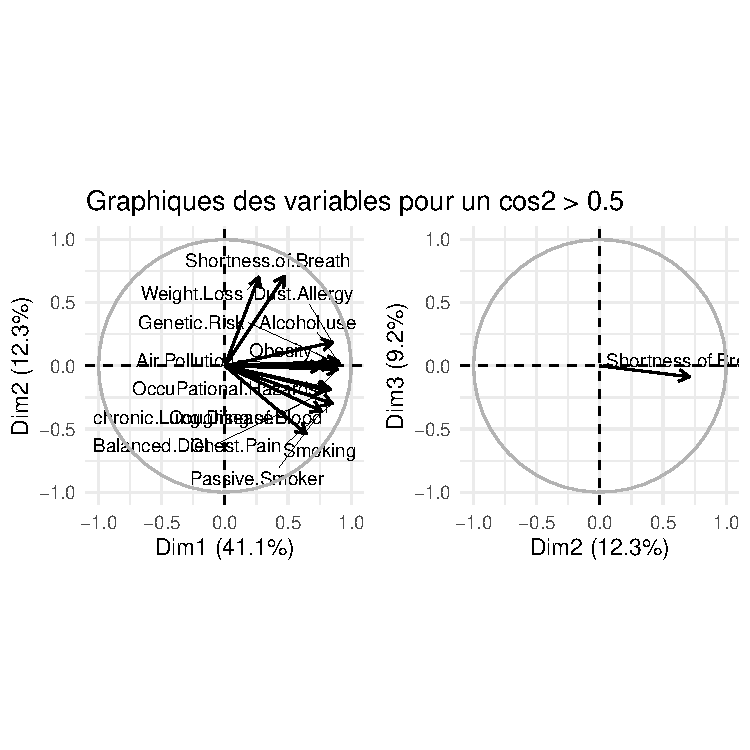
\includegraphics{dosfin-013}
\end{center}

On observe que, sur la dimension 1 et 2, de nombreuses variables semblent fortement corrélées, ce qui est en accord avec les résultats obtenus à partir de la matrice de corrélation. De plus, les flèches pointent majoritairement vers la droite, ce qui est cohérent avec la structure de nos données. En effet, les notes attribuées suivent une intensité croissante pour chaque variables Par conséquent, on peut supposer que, sur le plan 1 \& 2, plus un individu se situe à droite du plan, plus ses conditions de santé pourraient être considérées comme dégradées. 

En revanche, pour la dimension 2 et 3, seule une variable est bien représentée. Ainsi, nous avons décidé de l'ignorer pour la suite de l'analyse et de nous concentrer uniquement sur la dimension 1 et 2.

\newpage

\subsection{Nuage des individus}

Nous allons à présent projeter les individus sur les axes principaux afin d’observer si les variables utilisées permettent de distinguer visuellement des groupes d’individus. L’objectif est de vérifier si nos variables possèdent un pouvoir discriminant significatif, en particulier sur les dimensions 1 et 2 retenues précédemment.

\begin{center}
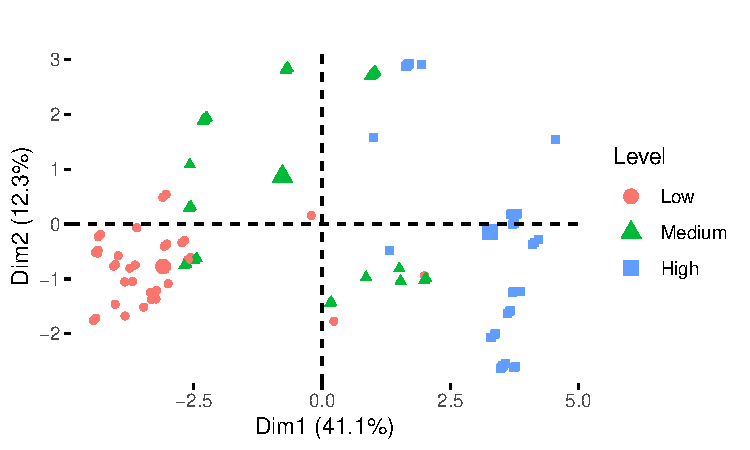
\includegraphics{dosfin-014}
\end{center}

On observe clairement sur ce graphique une séparation nette des trois classes, comme attendu : les individus présentant de fortes chances se situent à droite, tandis que ceux ayant de faibles chances se trouvent à gauche. Au vu de l’ensemble de nos analyses statistiques, nous pouvons conclure que notre jeu de données présente un fort pouvoir discriminant grâce aux variables sélectionnées. Ainsi, lorsqu’elles sont appliquées à des modèles prédictifs, même des approches simples comme le \textit{k}-plus proches voisins (\textit{k}-NN) peuvent s'avérer particulièrement performantes, compte tenu de la clarté des regroupements observés dans l’espace factoriel.

Toutefois, un enjeu important reste la capacité de généralisation de ces modèles à d’autres jeux de données, notamment si les distributions diffèrent sensiblement. Cette variabilité pourrait entraîner une baisse de performance. Néanmoins, le système de notation utilisé ici, en attribuant des niveaux d’intensité plutôt que des mesures précises, pourrait offrir une certaine robustesse face à ce type de variation, contrairement à des métriques médicales strictes.


\section{Création des modèles}

Dans cette section, nous allons appliquer différents modèles de classification à notre jeu de données, comparer leurs performances, puis sélectionner celui qui s’avère le plus optimal.


\subsection{Prétraitement}

Comme nous l’avons vu précédemment, notre jeu de données présente certain default, notamment des problèmes de corrélation entre variables ainsi que la présence de valeurs extrêmes dans la distribution de certaines d’entre elles, selon les classes à prédire.

Il est donc nécessaire de mettre en place des méthodes permettant de réduire au maximum ces problèmes, afin d’optimiser les performances de nos modèles et garantir une meilleure robustesse.

\subsubsection{Séparation des données}

Nous allons séparer notre jeu de données en deux sous-ensembles : les données d’entraînement, représentant 75\% de l’échantillon total, et les données de test, qui serviront à évaluer les performances de nos modèles.  
Afin de garantir une évaluation fiable, nous veillerons à conserver la même proportion des classes cibles dans ces deux ensembles.


\subsubsection{Recette}

\begin{Schunk}
\begin{Sinput}
> rec <- recipe(Level ~ ., data = data_train)
\end{Sinput}
\end{Schunk}
Nous allons prédire le risque d'avoir un cancer avec toutes nos autres variables.

\subsubsection{Corrélations}

\begin{Schunk}
\begin{Sinput}
> rec <- recipe(Level ~ ., data = data_train) %>%
+   step_corr(all_numeric_predictors(), threshold = tune())
\end{Sinput}
\end{Schunk}


Pour réduire le problème de corrélation, nous allons appliquer un prétraitement \textbf{spep\_corr}, qui permet, pour chaque paire de variables fortement corrélées, de ne conserver qu’une seule des deux.  
Cette sélection se fait en fonction d’un seuil de corrélation maximal admissible, que nous optimiserons au préalable. Ainsi, seules les variables apportant une information réellement distincte sont conservées.

\subsubsection{Valeurs extrèmes}

\begin{Schunk}
\begin{Sinput}
> rec <- recipe(Level ~ ., data = data_train)%>% 
+   
+   step_corr(all_numeric_predictors(), threshold = tune()) %>%
+   
+   step_outliers_maha(all_numeric(), -all_outcomes()) %>%
+   
+   step_outliers_lookout(all_numeric(),-contains(r"(.outliers)"),
+                         -all_outcomes()) %>% 
+   
+   step_outliers_remove(contains(r"(.outliers)"),
+                        score_dropout = tune("dropout"),
+                        aggregation_function = "mean")
\end{Sinput}
\end{Schunk}



Pour réduire l'impact des valeurs extrêmes sur certains de nos modèles, nous allons utiliser les prétraitements fournis par la bibliothèque \texttt{tidy.outlier}. Ce package permet de détecter et de traiter les valeurs extrèmes dans les données, ce qui est important pour assurer la bonne performance de nos modèles.

Les étapes suivantes seront appliquées à nos données :

\begin{itemize}
  \item \texttt{step\_outliers\_maha} : Cette étape permet d’identifier les valeurs aberrantes en utilisant la méthode de Mahalanobis. Elle est appliquée sur toutes les variables numériques tout en excluant les variables cibles (\texttt{outcomes}).
  
  \item \texttt{step\_outliers\_lookout} : Cette étape sert à repérer d'autres valeurs extrêmes, en excluant celles déjà marquées comme aberrantes par l'étape précédente. Elle s’applique également sur toutes les variables numériques.
  
  \item \texttt{step\_outliers\_remove} : Cette étape supprime les valeurs extrêmes identifiées dans les étapes précédentes. Elle permet de contrôler le niveau de suppression (\texttt{score\_dropout}) et choisit la méthode d’agrégation (ici, la moyenne) pour remplacer les valeurs extrêmes.
  
\end{itemize}


\subsection{Rééchantillonnage}

Dès lors que nous allons optimiser des paramètres, nous effectuons une validation croisée à 10 plis afin de conserver un équilibre entre biais et variance, contrairement à d'autres méthodes comme le bootstrap. Cette méthode permet d'évaluer la performance de notre modèle en utilisant différentes sous-parties du jeu de données pour l'entraînement et la validation, en en l'occurrence 10, ce qui garantit une meilleure estimation de la performance du modèle tout en évitant le surapprentissage.

\subsection{Methodes d'évaluations}

\subsubsection{Métriques}

Pour évaluer nos modèles nous allons nous appuyer sur différentes métriques:

\begin{table}[H]
\centering
\small
\renewcommand{\arraystretch}{1.2}
\begin{tabular}{|l|p{10cm}|}
\hline
\textbf{Métrique} & \textbf{Description} \\
\hline
\texttt{accuracy} & Mesure de la proportion des prédictions correctes par rapport au total des prédictions effectuées. Plus la valeur est élevée, meilleur est le modèle. \\
\texttt{f\_meas (macro)} & La moyenne de la mesure F1 pour chaque classe, traitée de manière égale. Elle combine la précision et le rappel. \\
\texttt{recall (macro)} & Moyenne du rappel pour chaque classe, calculée de manière égale. Le rappel mesure la capacité du modèle à identifier correctement les instances positives. \\
\texttt{precision (macro)} & Moyenne de la précision pour chaque classe. La précision mesure la proportion d'éléments correctement identifiés comme positifs parmi ceux classés comme positifs. \\
\texttt{spec (macro)} & Moyenne de la spécificité pour chaque classe, qui mesure la capacité du modèle à identifier correctement les instances négatives. \\
\texttt{roc\_auc (macro)} & Moyenne de l'aire sous la courbe ROC pour chaque classe. Cette métrique mesure la capacité du modèle à bien séparer les classes. \\
\hline
\end{tabular}
\caption{Description des métriques de performance utilisées pour évaluer le modèle.}
\end{table}

\subsubsection{Procédé d'évaluation}

Pour évaluer nos modèles, nous commencerons par afficher les paramètres optimaux retenus pour chaque modèle. Ensuite, un tableau récapitulatif des métriques mentionnées ci-dessus sera présenté pour chaque modèle, incluant l'erreur d'entraînement et d'évaluation, afin de vérifier la présence d'un potentiel overfitting.

Dans un deuxième temps, nous afficherons les courbes ROC pour évaluer la capacité du modèle à discriminer entre les classes. Enfin, une matrice de confusion sera présentée pour visualiser les performances de chaque modèle.

Pour le modèle d'arbre de décision, l'arbre sera affiché afin de mieux comprendre les décisions prises par le modèle. L'importance des variables sera également examinée pour l'arbre de décision, la forêt aléatoire et le boosting, afin de déterminer quelles caractéristiques ont le plus d'influence sur les prédictions.


\section{Création des modèles}

Dans cette section, nous allons procéder à l’évaluation des principales familles de modèles de classification sur notre jeu de données. Chaque modèle sera comparé selon un ensemble de métriques de performance définies précédemment. À l’issue de cette analyse, nous sélectionnerons le modèle offrant les meilleurs compromis entre performance, robustesse et interprétabilité.

\subsection{Analyse Discriminante Quadratique}

La QDA est un modèle de classification qui, contrairement à la version linéaire (LDA), autorise chaque classe à avoir sa propre matrice de covariance, ce qui permet de modéliser des frontières de décision non linéaires.

Nous commençons donc par ce modèle. Étant donné la forte corrélation présente dans notre jeu de données, il est possible que des problèmes apparaissent lors de l’inversion des matrices de variance-covariance propres à chaque classe. 

Nous allons optimiser notre recette de prétraitement spécifiquement pour ce modèle, puis la conserver inchangée pour l’ensemble des modèles testés. En effet, ce prétraitement supprime à la fois certaines variables et certains individus. Afin de garantir une équité entre tous les modèles évalués, il est essentiel qu’ils soient tous entraînés sur le même jeu de données transformé.

\subsubsection{Optimisation de la recette}

Nous allons optimiser notre QDA pour 5 valeurs de threshold comprises entre 0 et 1 et 10 valeurs de dropout comprisent entre 0 et 1



\begin{center}

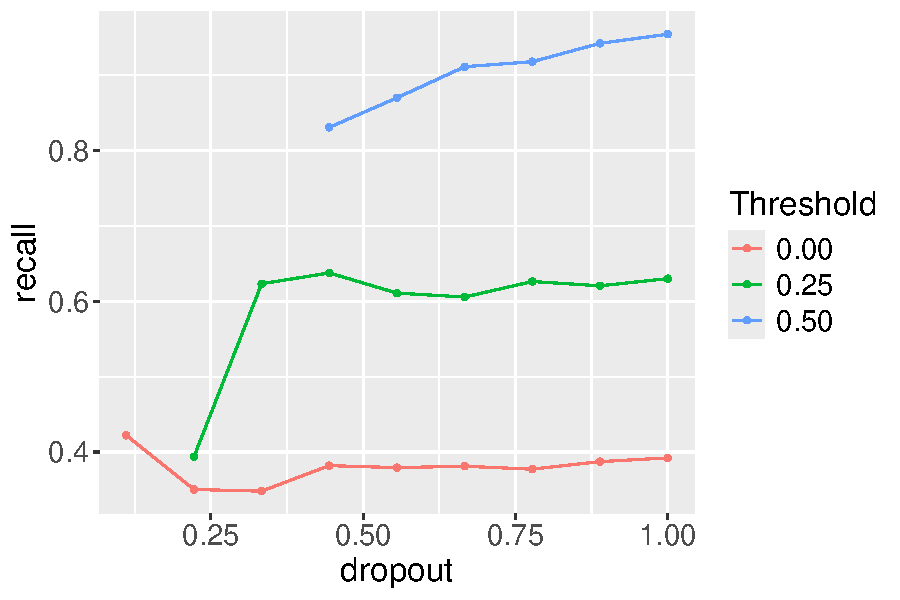
\includegraphics{dosfin-019}

Nous pouvons observer qu'au-delà d’un \textit{threshold} de 0{,}5, aucun point n’est visible en fonction des valeurs de \textit{dropout}. Cela confirme nos craintes : le modèle n’est pas parvenu à inverser la matrice de variance-covariance pour certaines classes, celles-ci étant trop singulières.
\newpage
Dans un second temps, nous constatons que plus le \textit{threshold} est élevé, plus le \textit{recall} (rappel) tend à augmenter. Pour explorer cette tendance plus en détail, nous allons réitérer notre expérience avec 10 valeurs de \textit{threshold} comprises entre 0{,}3 et 0{,}45, et 5 valeurs de \textit{dropout} différentes comprises entre 0 et 1.

\end{center}

\begin{center}

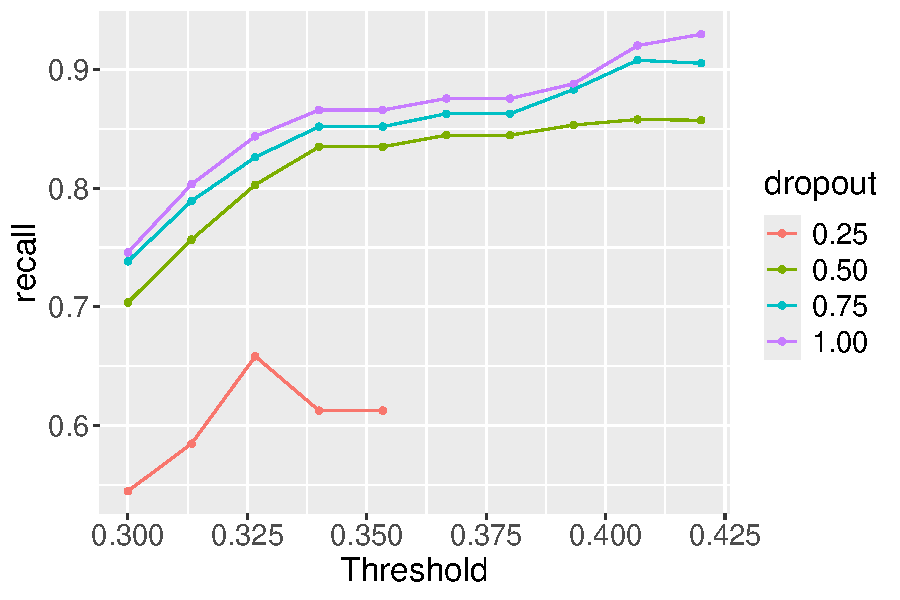
\includegraphics{dosfin-020}

% latex table generated in R 4.4.3 by xtable 1.8-4 package
% Sun Apr 20 03:37:04 2025
\begin{table}[ht]
\centering
\begin{tabular}{rrrllrrr}
  \hline
 & threshold & dropout & .metric & .estimator & mean & n & std\_err \\ 
  \hline
1 & 0.42000 & 1.00000 & recall & macro & 0.92964 &     10 & 0.00959 \\ 
  2 & 0.40667 & 1.00000 & recall & macro & 0.92007 &     10 & 0.01260 \\ 
  3 & 0.40667 & 0.75000 & recall & macro & 0.90774 &     10 & 0.01165 \\ 
  4 & 0.42000 & 0.75000 & recall & macro & 0.90519 &     10 & 0.00950 \\ 
  5 & 0.39333 & 1.00000 & recall & macro & 0.88791 &     10 & 0.01212 \\ 
   \hline
\end{tabular}
\caption{Meilleurs paramêtres} 
\end{table}
\end{center}


Au vu des résultats obtenus, et afin de minimiser l'erreur d'échantillonnage, nous retiendrons pour l'ensemble de nos modèles un \textit{threshold} de 0{,}42 et un \textit{dropout} de 0{,}75.


\newpage
\subsubsection{Résultat sur le modèle}

\begin{center}



% latex table generated in R 4.4.3 by xtable 1.8-4 package
% Sun Apr 20 03:37:04 2025
\begin{table}[ht]
\centering
\begin{tabular}{rlr}
  \hline
 & .metric & .estimate \\ 
  \hline
1 & accuracy & 90.00 \\ 
  2 & f\_meas & 90.10 \\ 
  3 & recall & 90.20 \\ 
  4 & precision & 90.00 \\ 
  5 & spec & 95.00 \\ 
  6 & roc\_auc & 98.80 \\ 
  7 & erreur\_test & 10.00 \\ 
  8 & erreur\_train & 9.90 \\ 
   \hline
\end{tabular}
\caption{Résultats} 
\end{table}
\end{center}


\subsubsection{Courbe ROC}

\begin{center}

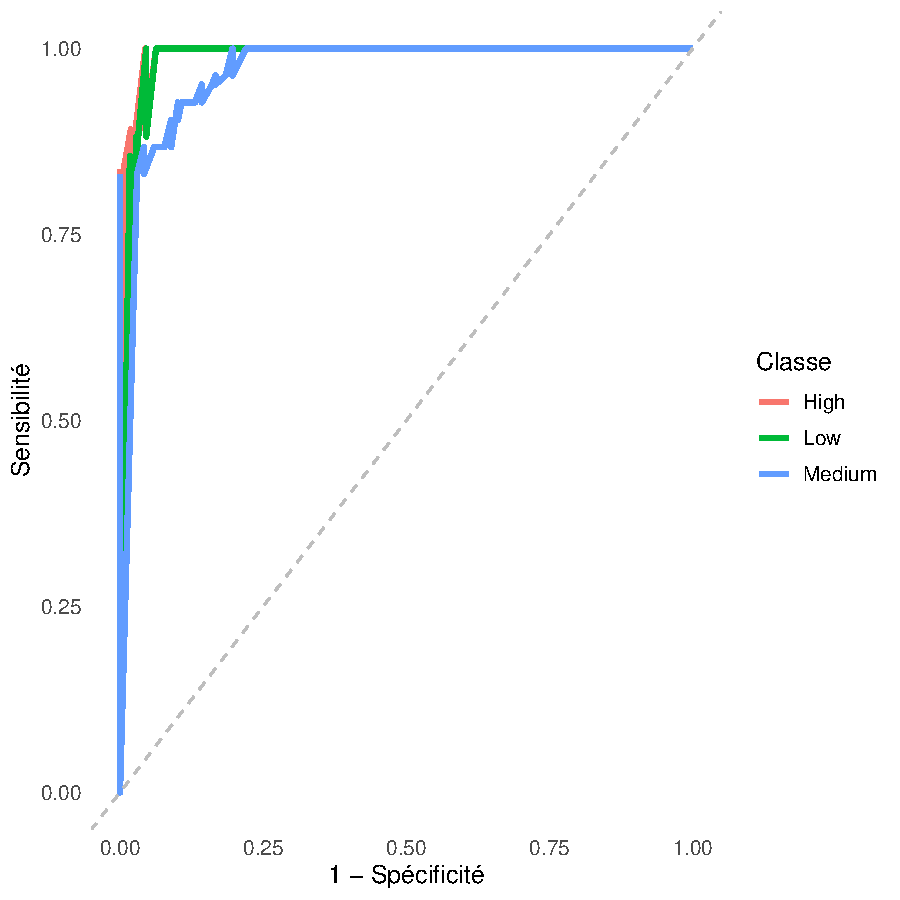
\includegraphics{dosfin-024}

\end{center}

\newpage

\subsubsection{Matrice de confusion}

\begin{center}

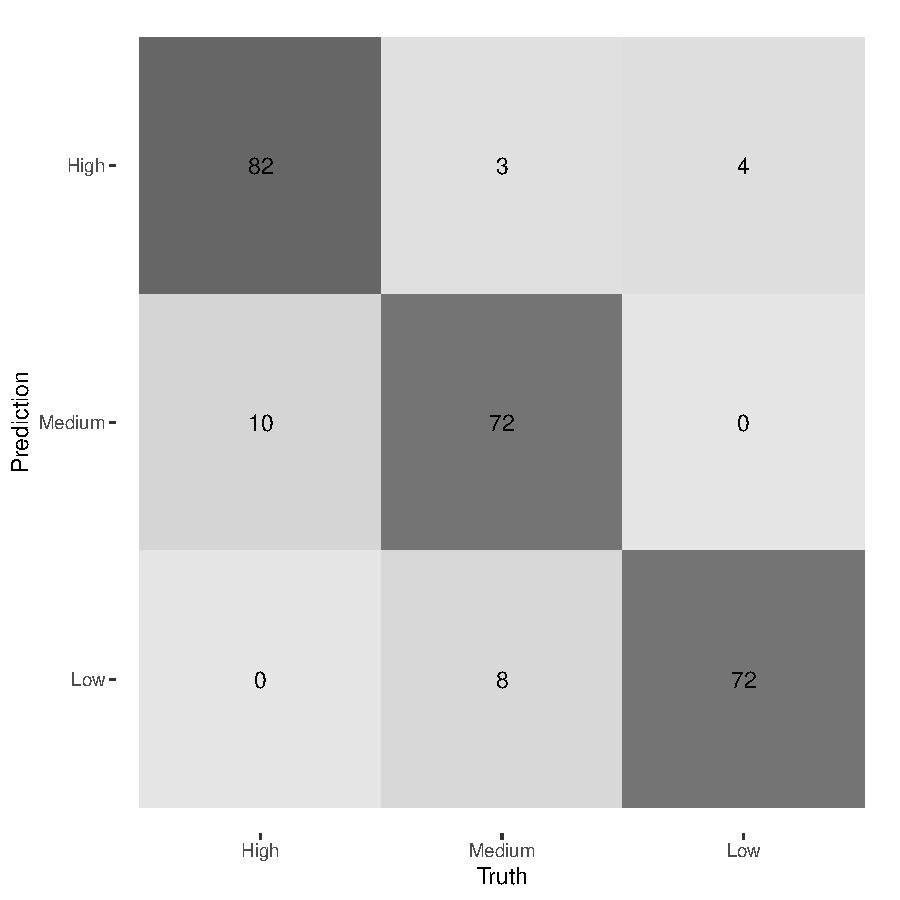
\includegraphics{dosfin-025}

\end{center}

\subsubsection{Interpretation}

Nous pouvons constater que la QDA est un très bon modèle, avec des métriques proches de 90\%. Comme prévu, ces bons résultats s'expliquent par la structure statistique de notre base de données. Les courbes ROC montrent une très bonne séparation entre les classes, bien que la classe \textit{médium} semble légèrement moins bien prédite. Ce constat est confirmé par la matrice de confusion, où cette classe présente le plus d'erreurs de classification.

Comme nous le verrons plus tard, ce modèle est l’un des moins performants. En effet, il repose sur l’hypothèse que les variables suivent une loi normale. Or, nos variables sont principalement quantitatives discrètes, ce qui les rend peu adaptées à une modélisation par une loi de probabilité continue. Cette inadéquation peut ainsi entraîner une baisse significative des performances du modèle.

\newpage

\subsection{Anylise Disctriminante Linéaire}

La LDA est un modèle de classification qui suppose que toutes les classes partagent une même matrice de covariance et que les variables suivent une distribution normal, ce qui impose des frontières de décision linéaires et en fait un modèle plus simple et plus robuste.


\subsubsection{Résultat sur le modèle}

\begin{center}


% latex table generated in R 4.4.3 by xtable 1.8-4 package
% Sun Apr 20 03:37:04 2025
\begin{table}[ht]
\centering
\begin{tabular}{rlr}
  \hline
 & .metric & .estimate \\ 
  \hline
1 & accuracy & 86.90 \\ 
  2 & f\_meas & 86.50 \\ 
  3 & recall & 86.60 \\ 
  4 & precision & 86.70 \\ 
  5 & spec & 93.40 \\ 
  6 & roc\_auc & 93.20 \\ 
  7 & erreur\_test & 13.10 \\ 
  8 & erreur\_train & 14.00 \\ 
   \hline
\end{tabular}
\caption{Résultats} 
\end{table}
\end{center}

\subsubsection{Courbe ROC}

\begin{center}

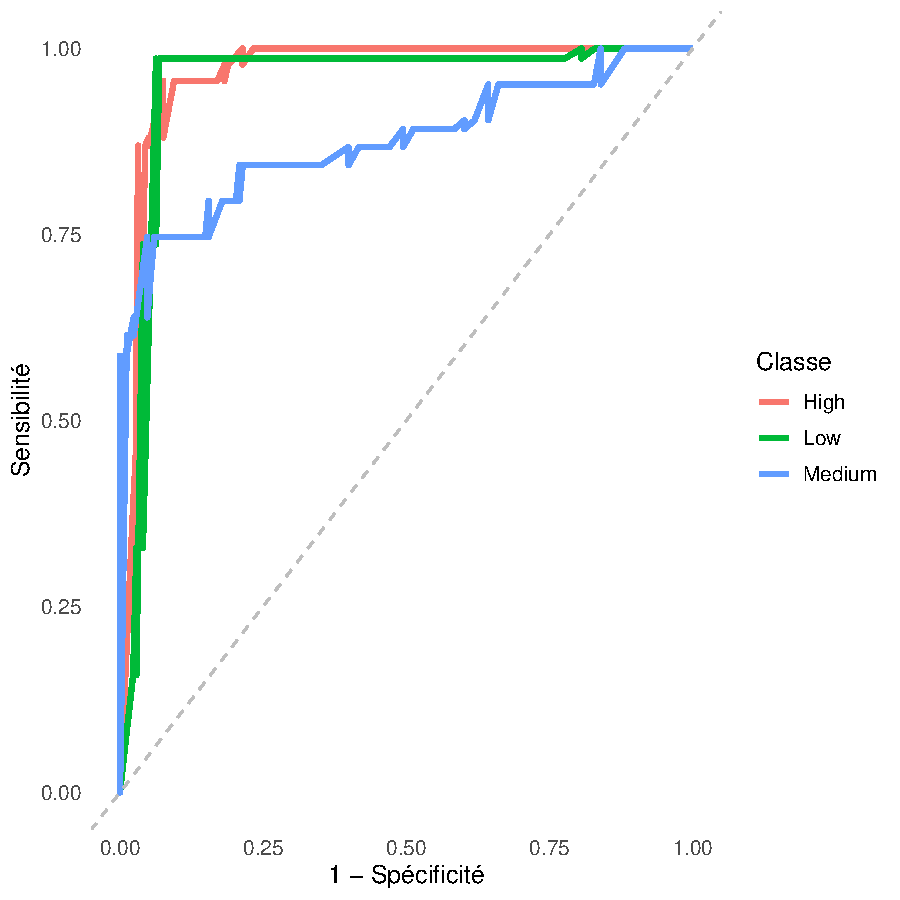
\includegraphics{dosfin-028}

\end{center}

\subsubsection{Matrice de confusion}

\begin{center}

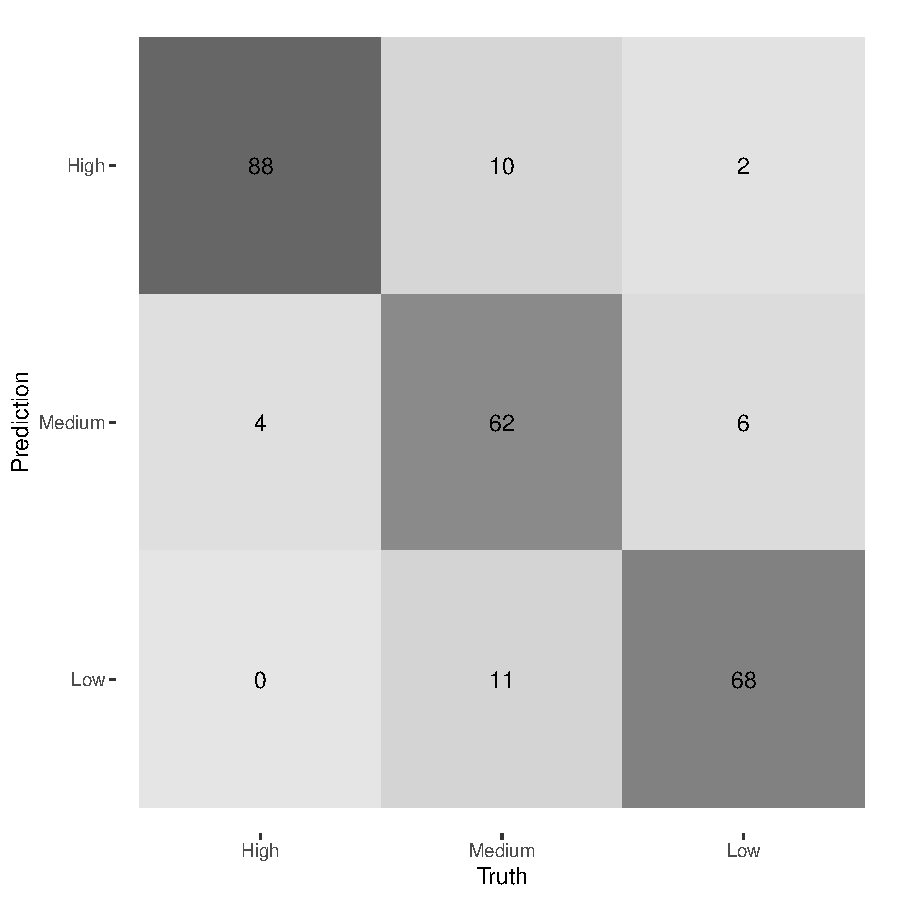
\includegraphics{dosfin-029}

\end{center}

\subsubsection{Interpretation}

Nous constatons que la \textbf{LDA} sous-performe par rapport à notre \textbf{QDA}, bien qu’elle affiche tout de même de bons scores avoisinant les \textbf{86\,\%} pour chacune des métriques. Cette contre-performance peut s’expliquer par le fait qu’aucune des hypothèses fondamentales de la LDA ne semble respectée dans notre jeu de données. D’un point de vue plus global, le modèle reste convenable, même si les courbes \textbf{ROC} révèlent une moins bonne distinction pour la classe \textit{Medium}, qui semble moins bien représentée.

\newpage


\subsection{k plus proches voisins}

Le modèle des k plus proches voisins est un algorithme de classification non paramétrique basé sur la proximité. Pour prédire la classe d'une nouvelle observation, le modèle recherche les k observations les plus proches dans l'espace des variables explicatives, puis attribue la classe majoritaire parmi ces voisins.

Ce modèle ne fait aucune hypothèse sur la distribution des données, ce qui le rend simple à mettre en œuvre mais sensible au choix du paramètre k. C'est pourquoi nous allons optimiser ce paramètre afin d'obtenir les meilleures performances possibles sur notre jeu de données.


\subsubsection{Optimisation des hyperparamêtres}



\begin{center}

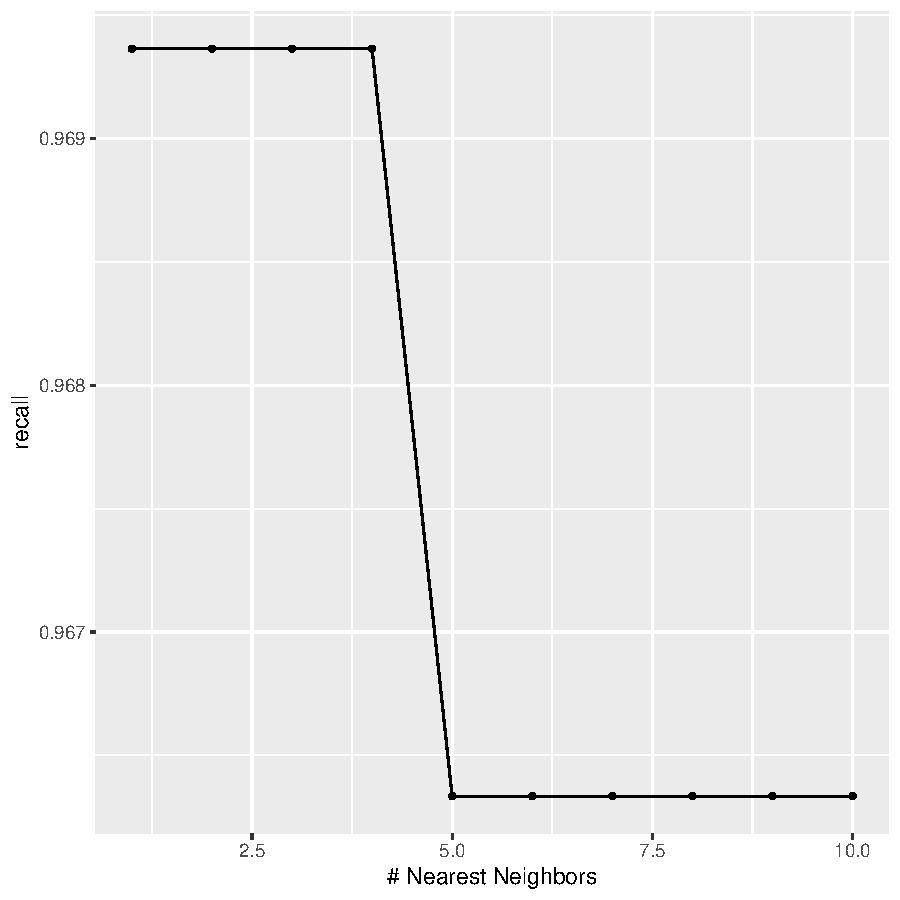
\includegraphics{dosfin-031}

\end{center}

Nous constatons que, pour un $k$ compris entre 1 et 4 inclus, les performances du modèle ne varient pas de manière significative au niveau du recall. Cela peut sembler surprenant au premier abord, notamment qu’un $k$ égal à 1 donne des résultats similaires à des valeurs plus élevées. Toutefois, compte tenu de la structure de nos données, qui sont parfaitement séparées, ce comportement devient logique.

Pour rappel, le paramètre $k$ détermine le nombre de voisins pris en compte par le modèle pour classifier une observation donnée.

\newpage

\subsubsection{Résultat sur le modèle}

\begin{center}


% latex table generated in R 4.4.3 by xtable 1.8-4 package
% Sun Apr 20 03:37:05 2025
\begin{table}[ht]
\centering
\begin{tabular}{rlr}
  \hline
 & .metric & .estimate \\ 
  \hline
1 & accuracy & 96.80 \\ 
  2 & f\_meas & 96.70 \\ 
  3 & recall & 96.80 \\ 
  4 & precision & 96.80 \\ 
  5 & spec & 98.40 \\ 
  6 & roc\_auc & 97.60 \\ 
  7 & erreur\_test & 3.20 \\ 
  8 & erreur\_train & 3.00 \\ 
   \hline
\end{tabular}
\caption{Résultats} 
\end{table}
\end{center}

\subsubsection{Courbe ROC}

\begin{center}

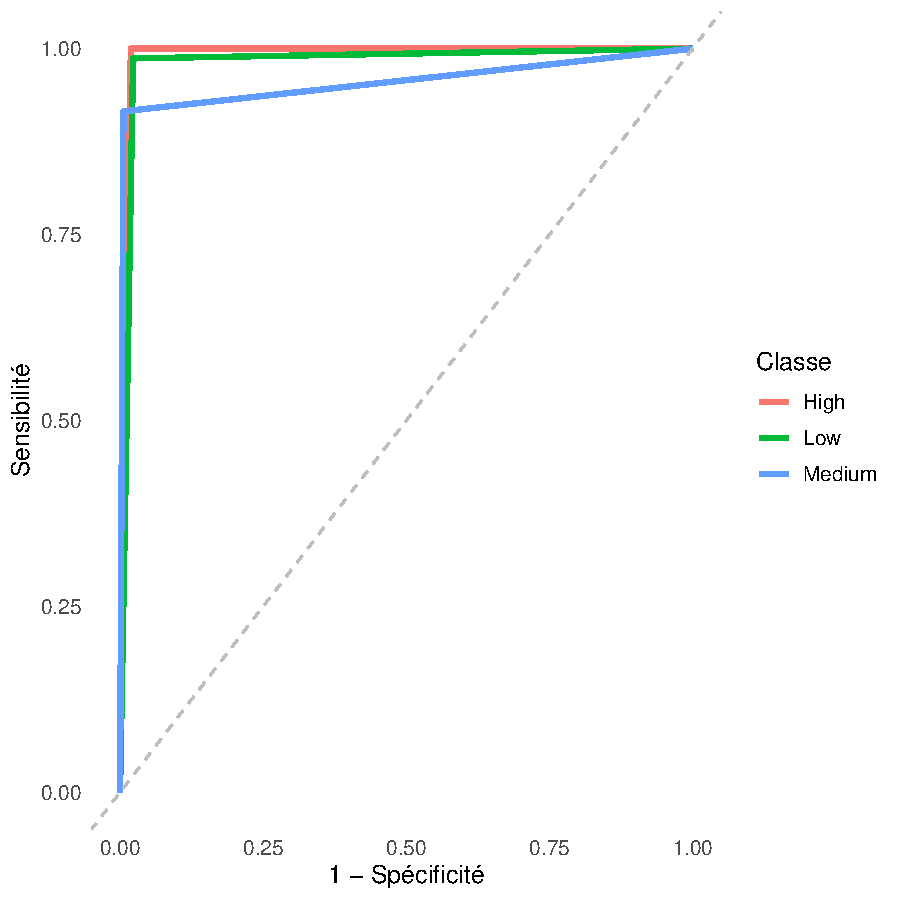
\includegraphics{dosfin-033}

\end{center}

\subsubsection{Matrice de confusion}

\begin{center}

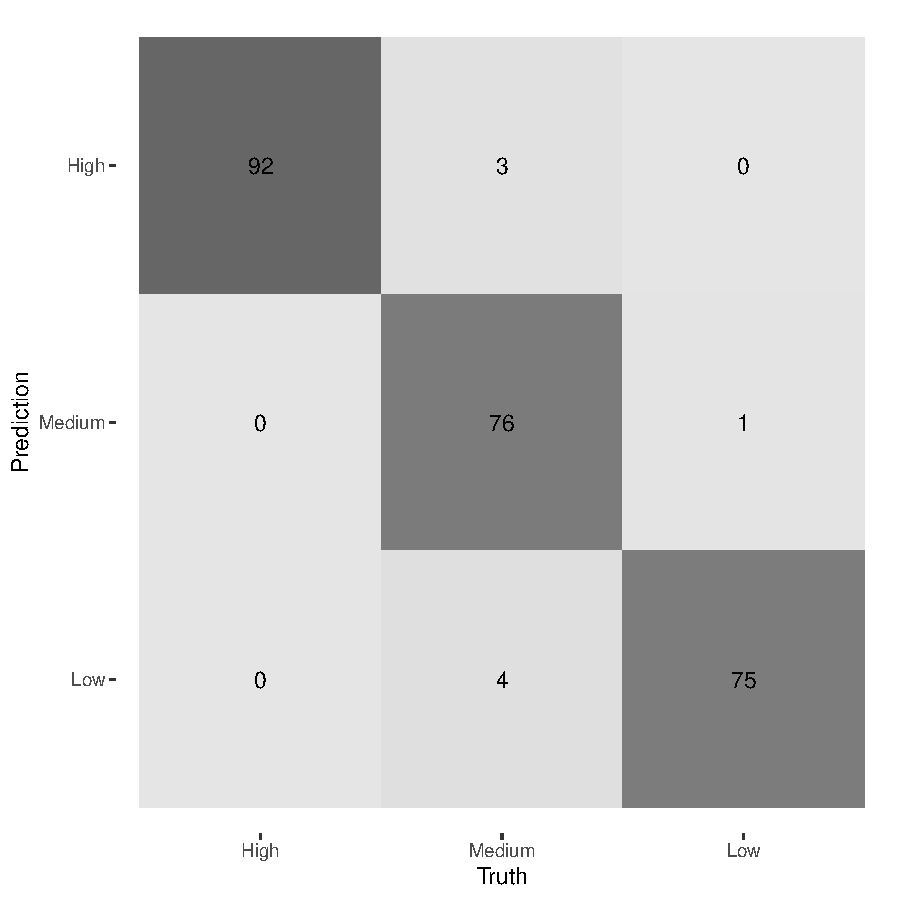
\includegraphics{dosfin-034}

\end{center}

\subsubsection{Interprétation}

Comme mentionné précédemment, grâce à notre jeu de données extrêmement bien séparé statistiquement, même un modèle simple comme le k-NN parvient à très bien classer nos individus, avec des scores moyens avoisinant les 96--97\,\%.

Les courbes ROC sont quant à elles très anguleuses, ce qui indique que le modèle est presque certain de ses prédictions. En revanche, la classe \textit{Medium} semble être la moins bien prédite, ce qui se reflète dans la matrice de confusion. À ce stade, nous ne disposons pas encore d’un modèle fiable pour prédire correctement cette classe.

\newpage

\subsection{Bayesien naïf}

Le classifieur bayésien naïf repose sur le théorème de Bayes, en supposant que les variables explicatives sont conditionnellement indépendantes entre elles et suivent une distribution normal, ce qui simplifie fortement le calcul des probabilités. Ce modèle est particulièrement efficace lorsque cette hypothèse est raisonnablement respectée.

Nous optimisons ici le paramètre de lissage (smoothness), qui permet d’éviter les probabilités nulles dans le cas où certaines combinaisons de variables n’apparaissent pas dans l’échantillon d’apprentissage. Ce lissage stabilise ainsi le modèle, notamment en présence de classes ou de modalités rares.

\subsubsection{Optimisation des hyperparamêtres}



\begin{center}

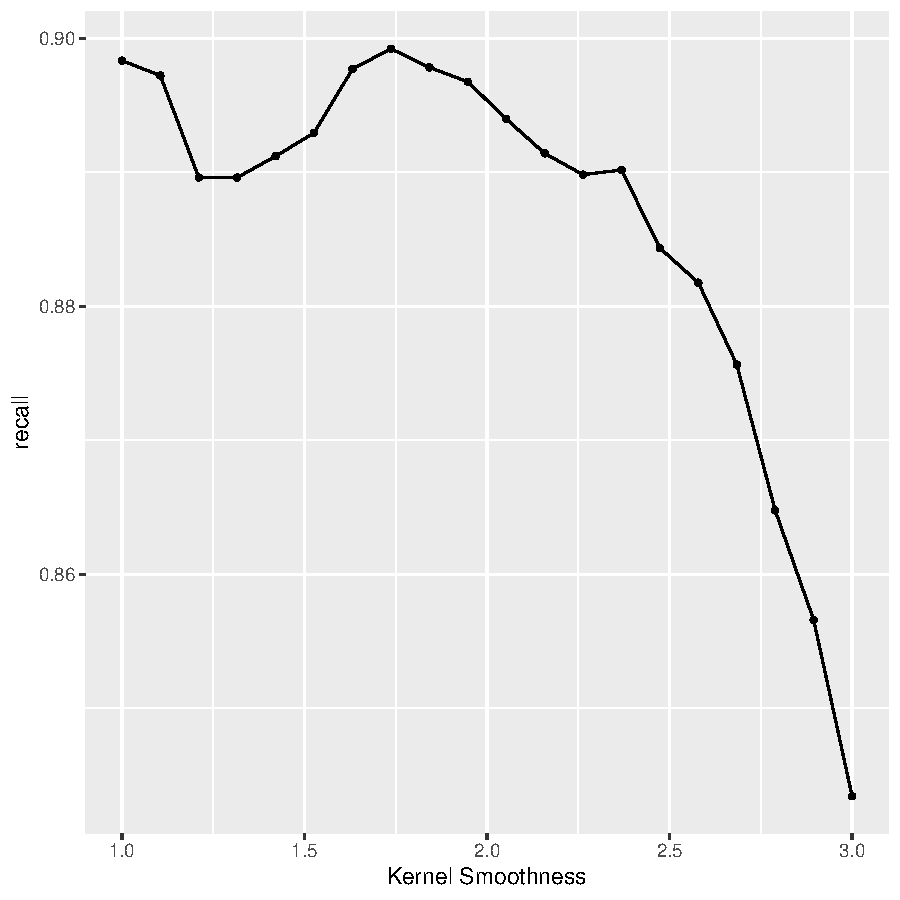
\includegraphics{dosfin-036}

\end{center}

Le paramètre qui maximise notre rappel est égal à 1.736842.


\newpage

\subsubsection{Résultat sur le modèle}

\begin{center}


% latex table generated in R 4.4.3 by xtable 1.8-4 package
% Sun Apr 20 03:37:06 2025
\begin{table}[ht]
\centering
\begin{tabular}{rlr}
  \hline
 & .metric & .estimate \\ 
  \hline
1 & accuracy & 90.00 \\ 
  2 & f\_meas & 89.50 \\ 
  3 & recall & 89.90 \\ 
  4 & precision & 91.20 \\ 
  5 & spec & 95.00 \\ 
  6 & roc\_auc & 93.90 \\ 
  7 & erreur\_test & 10.00 \\ 
  8 & erreur\_train & 9.00 \\ 
   \hline
\end{tabular}
\caption{Résultats} 
\end{table}
\end{center}

\subsubsection{Courbe ROC}

\begin{center}

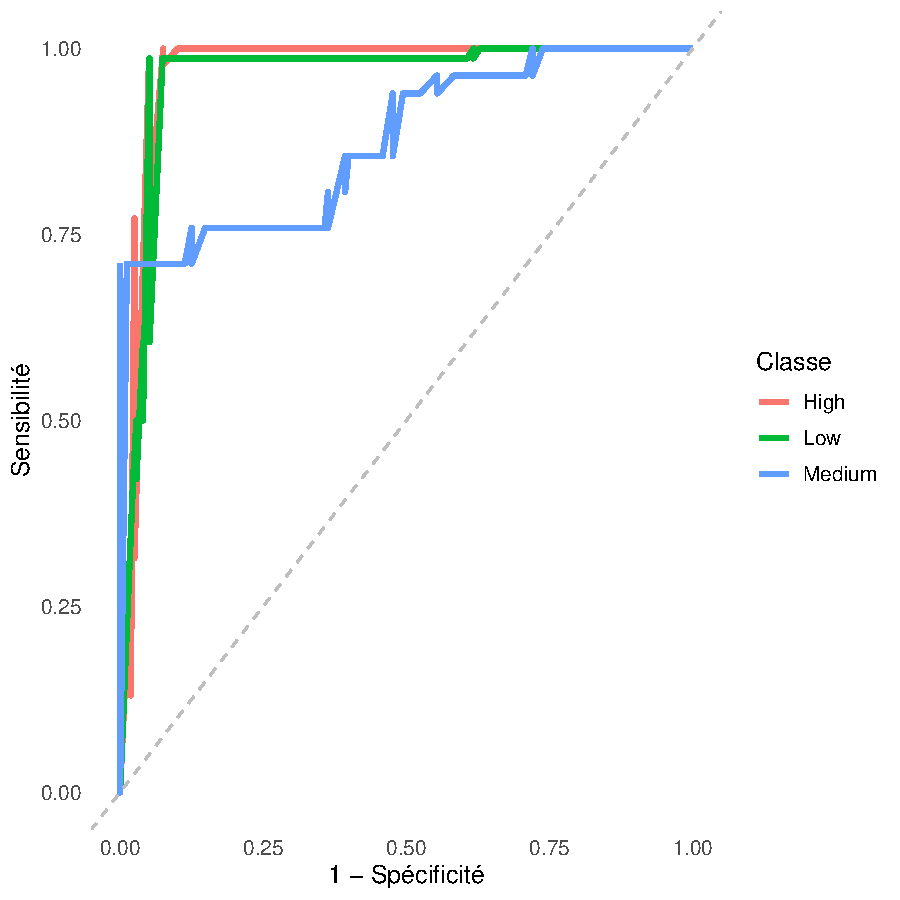
\includegraphics{dosfin-038}

\end{center}

\subsubsection{Matrice de confusion}

\begin{center}

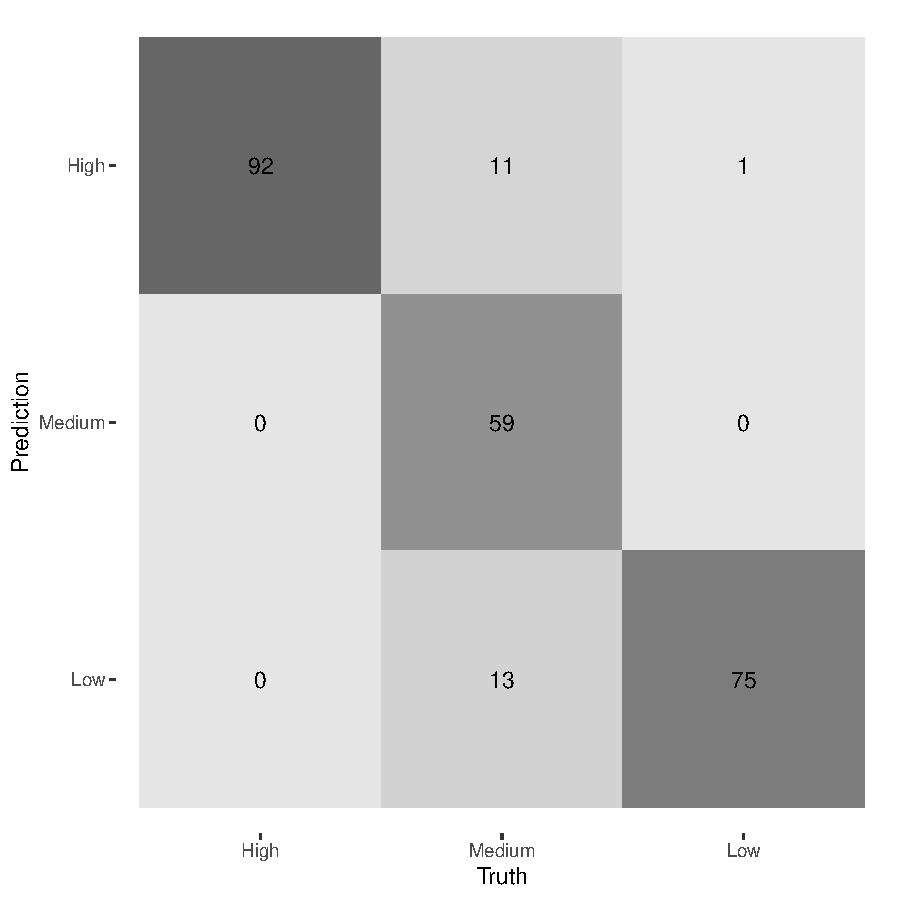
\includegraphics{dosfin-039}

\end{center}

\subsubsection{Interprétation}

Ce modèle nous offre des performances convenables mais relativement faibles en comparaison à nos autres modèles, avec une moyenne des métriques d’environ 90\%. Cela peut s’expliquer notamment par le fait que l’hypothèse de normalité et d'indépendance des variables ne sont pas respectées, ce qui peut entraîner une baisse de précision ou introduire un biais dans le modèle.


\newpage

\subsection{Support vecteur machine linéaire}

Le classifieur SVM linéaire cherche à séparer les classes à l’aide d’un hyperplan optimal maximisant la marge entre les observations de différentes classes. Ce modèle est particulièrement adapté lorsque les données sont linéairement séparables ou presque.

Nous optimisons ici le paramètre de coût, qui contrôle le compromis entre une séparation stricte des classes et l’autorisation de certaines erreurs de classification. Un coût élevé pénalise fortement les erreurs, tandis qu’un coût plus faible permet une marge plus large, au prix d’une tolérance aux erreurs.


\subsubsection{Optimisation des hyperparamêtres}



\begin{center}

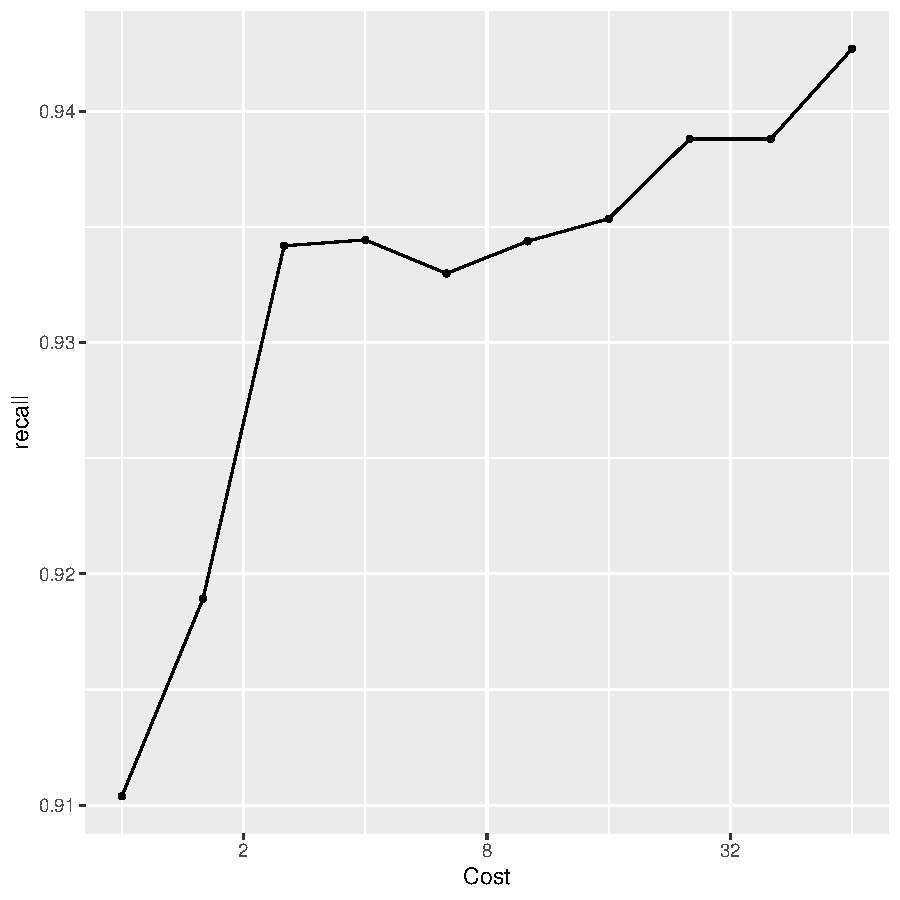
\includegraphics{dosfin-041}

\end{center}

Le coût qui maximise notre rappel est égal à 64. On observe que, de manière générale, plus le coût augmente, plus le modèle semble précis dans la détection des vrais positifs. Cependant, afin d’éviter de rendre notre modèle trop rigide face aux données d’apprentissage, nous choisissons de ne pas aller au-delà de cette valeur.



\newpage

\subsubsection{Résultat sur le modèle}

\begin{center}


% latex table generated in R 4.4.3 by xtable 1.8-4 package
% Sun Apr 20 03:37:07 2025
\begin{table}[ht]
\centering
\begin{tabular}{rlr}
  \hline
 & .metric & .estimate \\ 
  \hline
1 & accuracy & 93.20 \\ 
  2 & f\_meas & 93.30 \\ 
  3 & recall & 93.00 \\ 
  4 & precision & 94.00 \\ 
  5 & spec & 96.50 \\ 
  6 & roc\_auc & 96.30 \\ 
  7 & erreur\_test & 6.80 \\ 
  8 & erreur\_train & 5.10 \\ 
   \hline
\end{tabular}
\caption{Résultats} 
\end{table}
\end{center}

\subsubsection{Courbe ROC}

\begin{center}

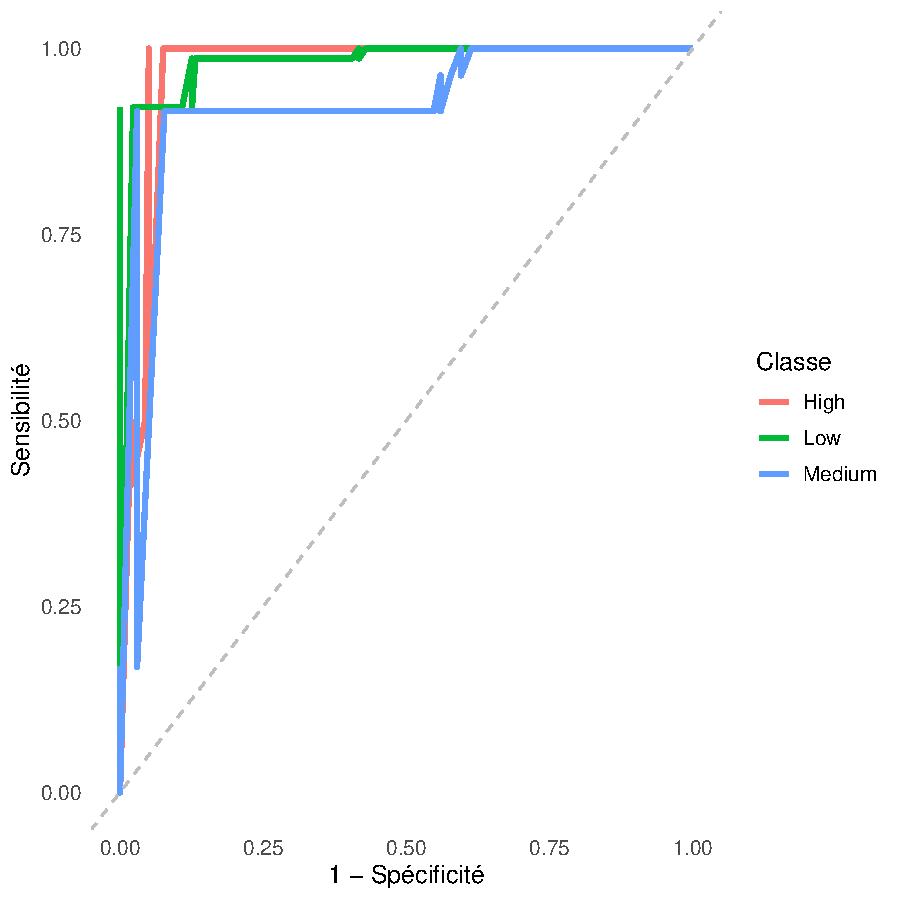
\includegraphics{dosfin-043}

\end{center}

\subsubsection{Matrice de confusion}

\begin{center}

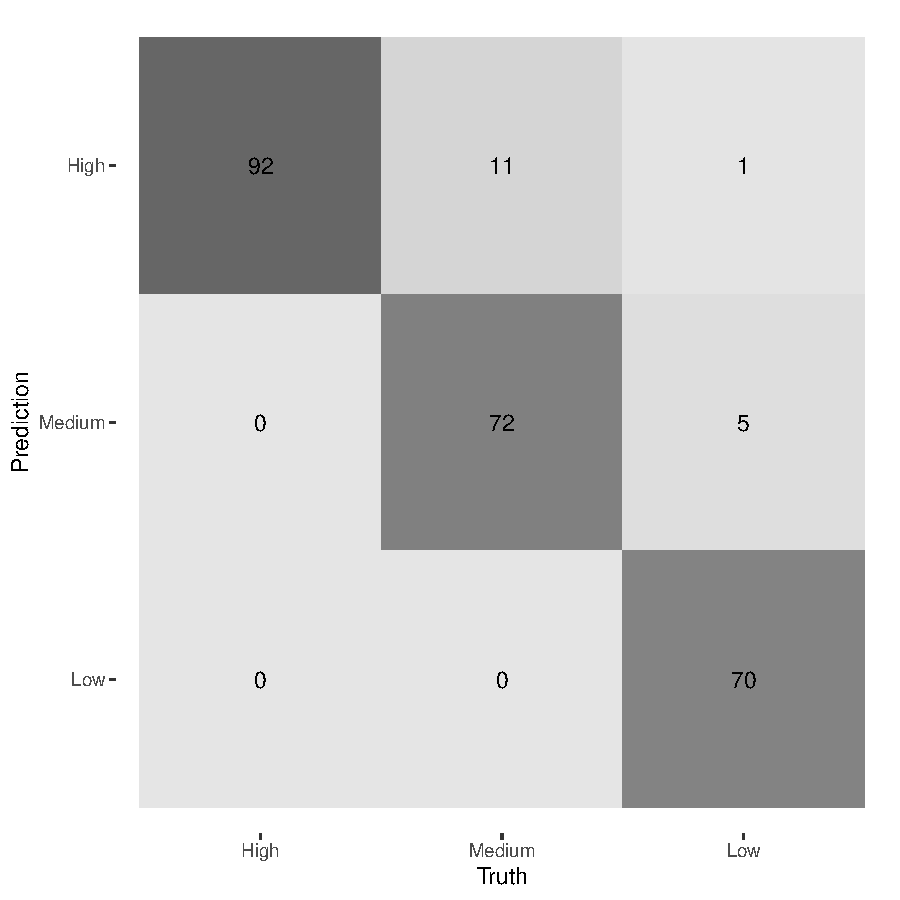
\includegraphics{dosfin-044}

\end{center}

\subsubsection{Interprétation}

Nous constatons des métriques toujours aussi bonnes, autour des 93\,\%, mais le modèle reste légèrement moins performant que la QDA. Cela peut suggérer que le jeu de données est peut-être moins bien séparable de manière linéaire. Pour valider cette hypothèse, nous examinerons dans la section suivante si elle semble réaliste à l’aide d’un SVM à noyau radial.

Par ailleurs, la classe médium reste la moins bien prédite parmi les trois classes.

\newpage

\subsection{Support vecteur machine radial}

Le classifieur SVM à noyau radial permet de modéliser des frontières de décision non linéaires en projetant les données dans un espace de dimension supérieure. Ce modèle est particulièrement efficace lorsque les classes ne sont pas linéairement séparables.

Nous optimisons ici les paramètres de coût et de largeur de noyau. Comme pour le modèle linéaire, le paramètre cost contrôle le compromis entre une séparation stricte et la tolérance aux erreurs.

Le paramètre sigma, quant à lui, détermine l’influence d’une observation individuelle : une valeur faible de sigma donne une frontière plus complexe et locale (risque de surapprentissage), tandis qu’une valeur plus grande produit une séparation plus lissée, moins sensible au bruit.



\subsubsection{Optimisation des hyperparamêtres}



\begin{center}

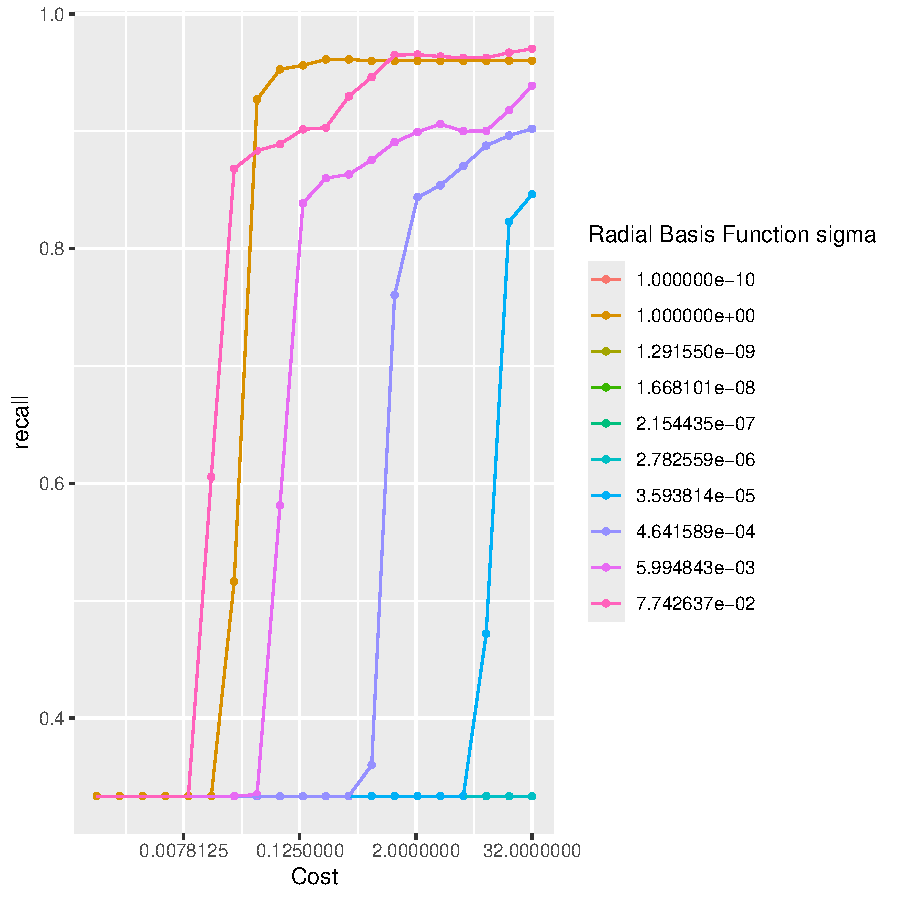
\includegraphics{dosfin-046}

\end{center}

Nous choisirons ici un coût de 32 avec un sigma de 0{,}0774264 afin de maximiser notre recall.  
Nous pourrions également tester des valeurs de coût plus élevées, mais les performances étant déjà très convenables, nous estimons que cela n’est pas nécessaire.  
D’autant plus que l’augmentation du coût ne semble pas apporter d’amélioration significative du recall.


\newpage

\subsubsection{Résultat sur le modèle}

\begin{center}


% latex table generated in R 4.4.3 by xtable 1.8-4 package
% Sun Apr 20 03:37:08 2025
\begin{table}[ht]
\centering
\begin{tabular}{rlr}
  \hline
 & .metric & .estimate \\ 
  \hline
1 & accuracy & 96.40 \\ 
  2 & f\_meas & 96.50 \\ 
  3 & recall & 96.50 \\ 
  4 & precision & 96.60 \\ 
  5 & spec & 98.20 \\ 
  6 & roc\_auc & 99.80 \\ 
  7 & erreur\_test & 3.60 \\ 
  8 & erreur\_train & 3.00 \\ 
   \hline
\end{tabular}
\caption{Résultats} 
\end{table}
\end{center}

\subsubsection{Courbe ROC}

\begin{center}

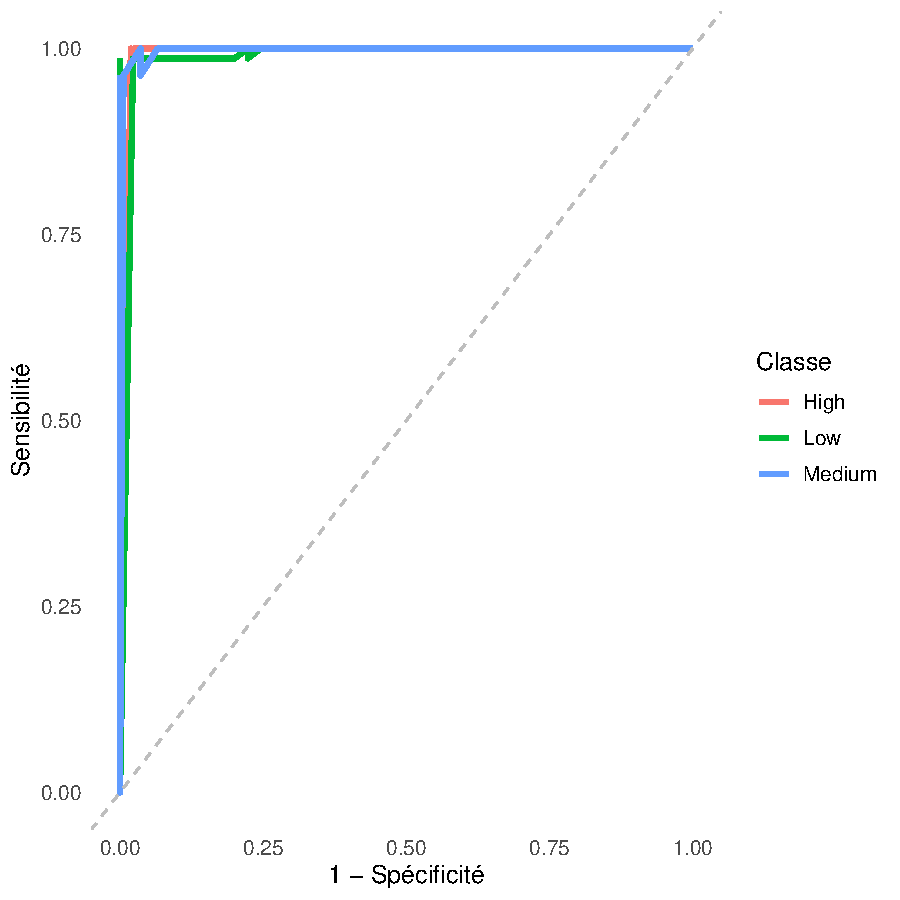
\includegraphics{dosfin-048}

\end{center}

\subsubsection{Matrice de confusion}

\begin{center}

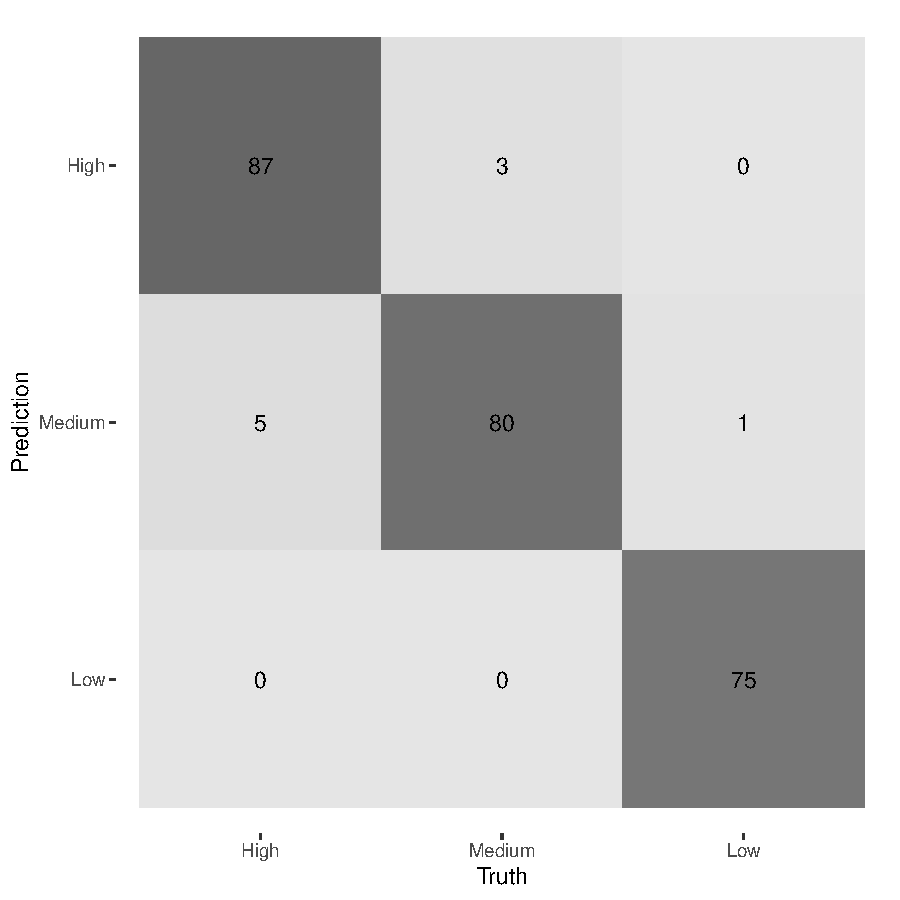
\includegraphics{dosfin-049}

\end{center}

\subsubsection{Interprétation}

Nous avons ici notre meilleur modèle en termes de performances, avec des métriques avoisinant en moyenne les 96\,\%.  
De plus, la courbe ROC montre que, pour la première fois, la classe \textit{Medium} est relativement bien prédite, ce qui se reflétera dans la matrice de confusion.

Nous pouvons ainsi conclure que, bien que le jeu de données discrimine fortement les classes en fonction des variables, il présente des difficultés avec une séparation linéaire.  
La structure sous-jacente des données semble indiquer que la séparation entre les classes est plus complexe, ce qui est bien illustré par l'efficacité du SVM à noyau radial.

\newpage

\subsection{Arbre de décision}

L’avantage de ce type de modèle est sa simplicité de compréhension.  
L’arbre de décision segmente l’espace des données en fonction des variables, à chaque nœud, dans le but de minimiser l’hétérogénéité des sous-groupes créés.  
Pour cela, nous utilisons l’entropie comme critère de division, une mesure qui quantifie le degré d’hétérogénéité d’un échantillon : plus l’entropie est faible, plus les observations sont similaires dans une même feuille.

Nous allons ici optimiser deux hyperparamètres :  
le coût de complexité, qui permet de pénaliser les arbres trop profonds ou trop détaillés afin de limiter le surapprentissage,  
et la profondeur maximale de l’arbre, qui restreint le nombre de divisions possibles, évitant ainsi une modélisation trop spécifique du bruit présent dans les données.



\subsubsection{Optimisation des hyperparamêtres}



\begin{center}

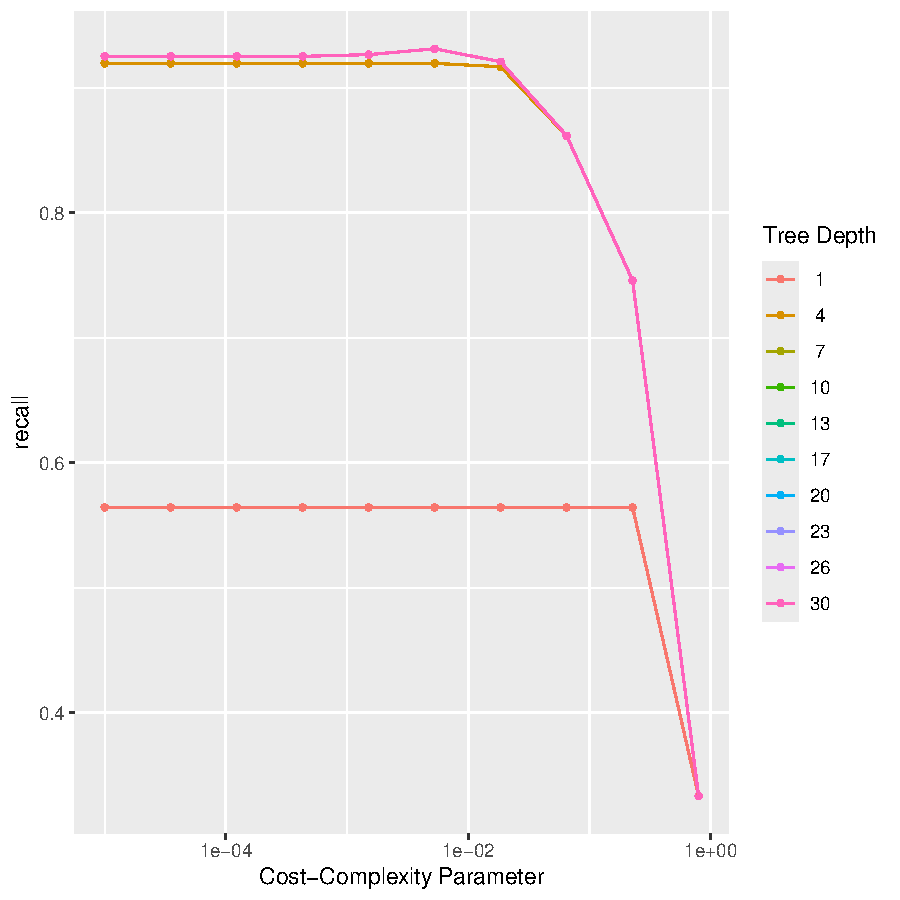
\includegraphics{dosfin-051}

\end{center}

Nous pouvons observer que, plus le coût de complexité augmente, plus le recall diminue.  
Cela s’explique par le fait qu’un coût plus élevé pénalise fortement les arbres complexes, ce qui conduit à des modèles plus simples et donc potentiellement moins sensibles à certaines classes.

Les hyperparamètres finalement retenus sont un coût de complexité de 0{,}005275 et une profondeur maximale de 7.



\newpage

\subsubsection{Résultat sur le modèle}

\begin{center}


% latex table generated in R 4.4.3 by xtable 1.8-4 package
% Sun Apr 20 03:37:09 2025
\begin{table}[ht]
\centering
\begin{tabular}{rlr}
  \hline
 & .metric & .estimate \\ 
  \hline
1 & accuracy & 93.60 \\ 
  2 & f\_meas & 93.30 \\ 
  3 & recall & 93.20 \\ 
  4 & precision & 93.50 \\ 
  5 & spec & 96.80 \\ 
  6 & roc\_auc & 98.30 \\ 
  7 & erreur\_test & 6.40 \\ 
  8 & erreur\_train & 5.00 \\ 
   \hline
\end{tabular}
\caption{Résultats} 
\end{table}
\end{center}

\subsubsection{Courbe ROC}

\begin{center}

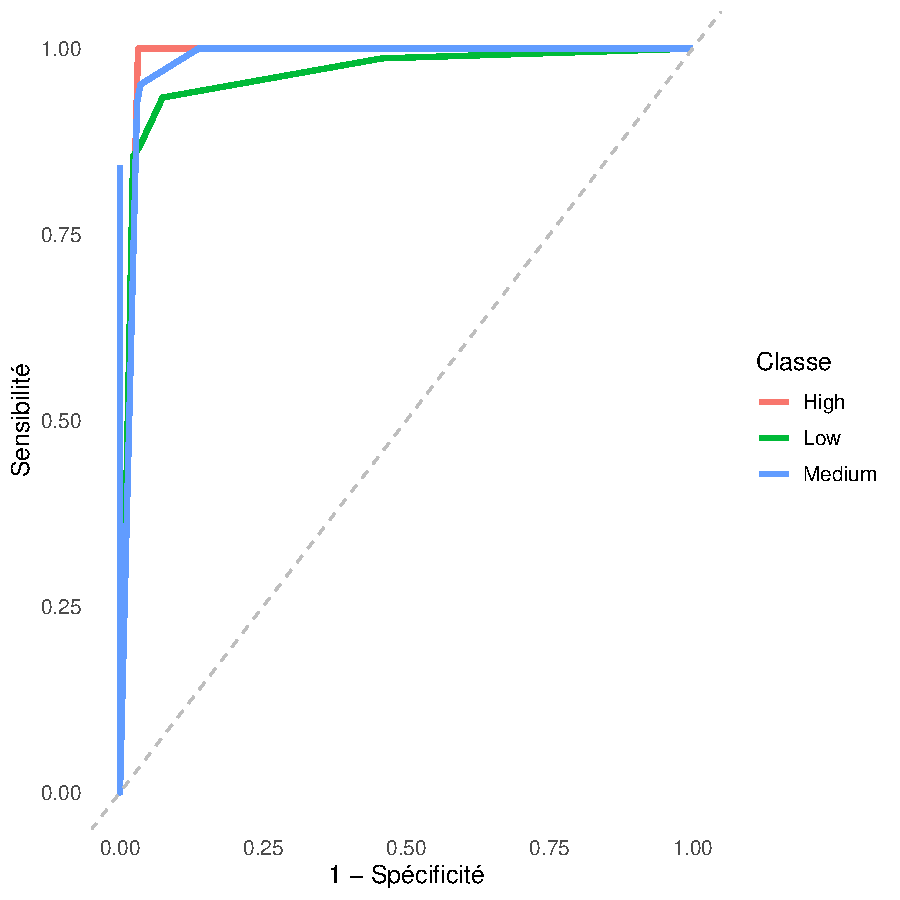
\includegraphics{dosfin-053}

\end{center}

\subsubsection{Matrice de confusion}

\begin{center}

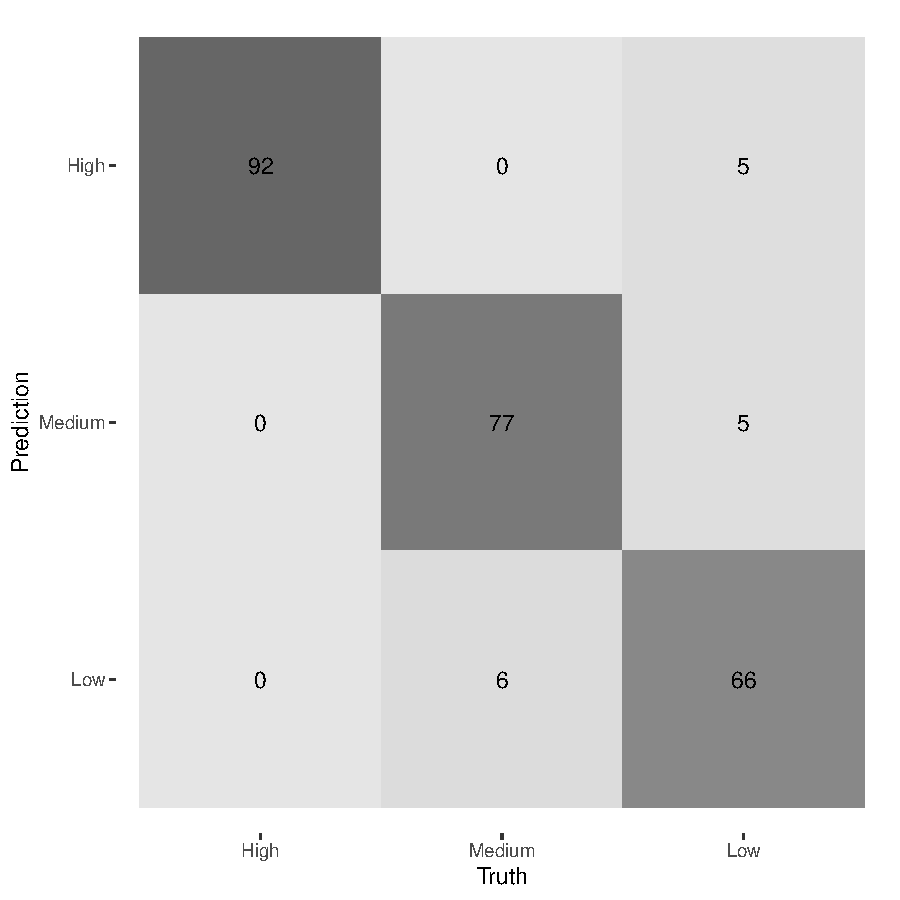
\includegraphics{dosfin-054}

\end{center}


\subsubsection{Arbre}

\begin{center}

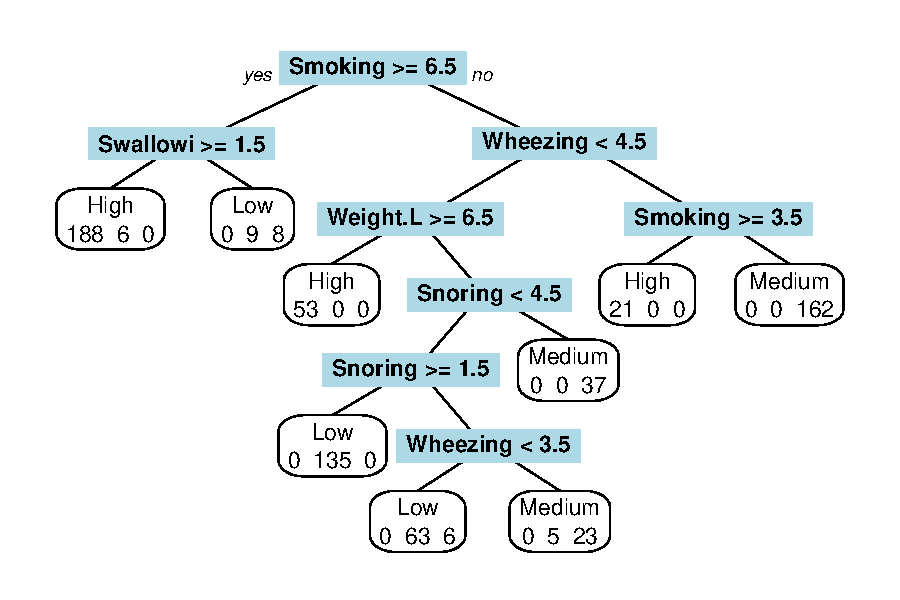
\includegraphics{dosfin-055}

\end{center}

\subsubsection{Importance des variables}

\begin{center}

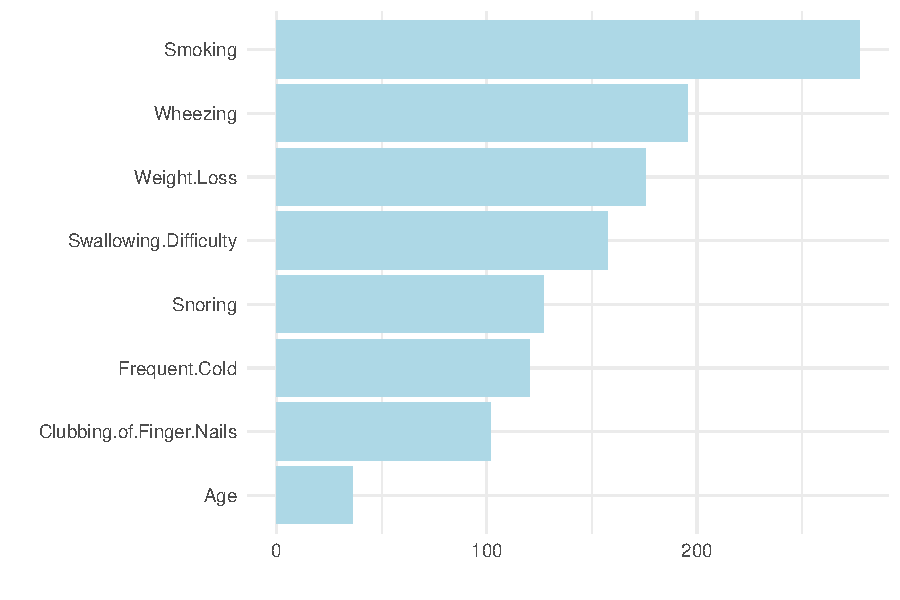
\includegraphics{dosfin-056}

\end{center}

\subsubsection{Interprétation}

Notre arbre de décision obtient de très bons résultats, avec des performances avoisinant les 93\,\%.  
Cependant, il reste légèrement moins performant que le SVM radial, ce qui peut s’expliquer par la capacité limitée de l’arbre à modéliser des relations complexes entre les variables.

Selon les courbes ROC, la classe Medium est ici mieux prédite que dans les autres modèles, ce qui suggère que l’arbre de décision parvient à mieux capter certaines structures spécifiques liées à cette classe.

L’arbre retenu présente une complexité équilibrée : il n’est ni trop court (ce qui aurait mené à un underfitting), ni trop profond (risque de overfitting).

Enfin, en ce qui concerne l’importance des variables, aucune ne semble dominer significativement les autres.  
À noter que la variable Age est l’une des moins utilisées, ce qui est cohérent avec les analyses exploratoires menées précédemment.

\newpage

\subsection{Forêt aléatoire}

La forêt aléatoire combine plusieurs arbres de décision afin d'améliorer la stabilité et la performance du modèle tout en limitant le surapprentissage.  
Chaque arbre est construit à partir d’un échantillon bootstrapé, avec une sélection aléatoire de variables à chaque division, ce qui augmente la diversité.

Trois hyperparamètres sont optimisés : le mtry (nombre de variables testées à chaque division), la profondeur maximale des arbres (pour limiter leur complexité), et le min\_n (nombre minimal d'observations dans un nœud avant division).  

Ce modèle est robuste face aux variations des données et conserve une certaine interprétabilité via l’analyse de l’importance des variables.



\subsubsection{Optimisation des hyperparamêtres}



\begin{center}

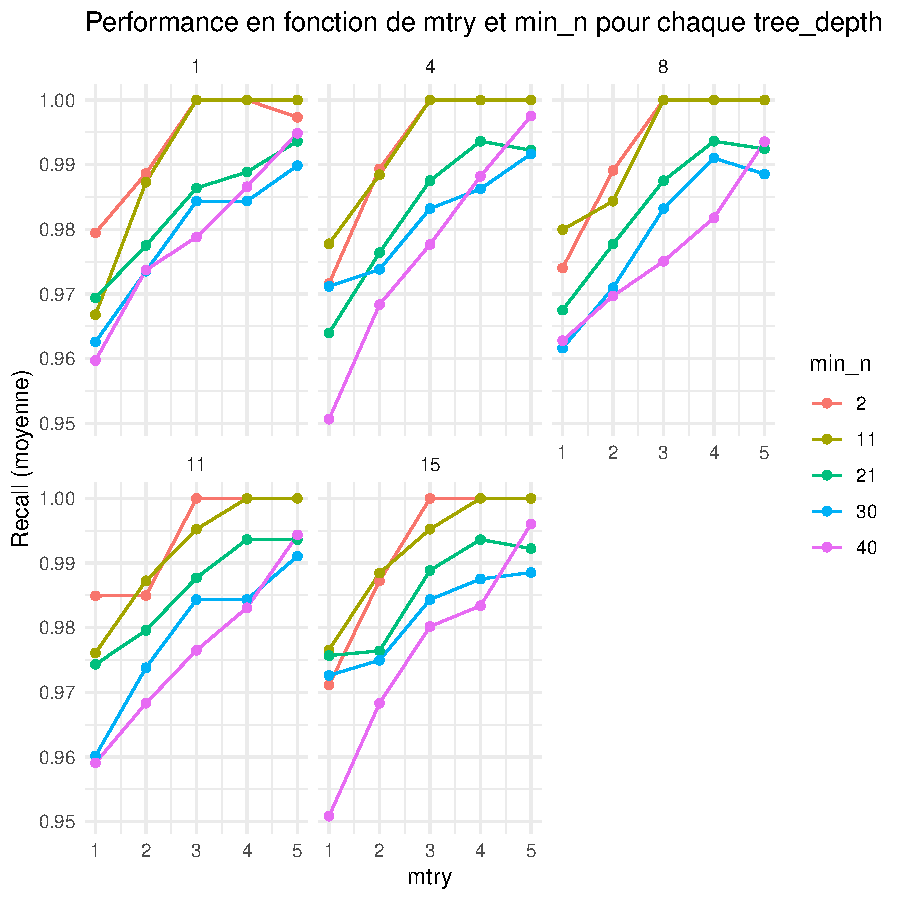
\includegraphics{dosfin-058}

\end{center}

On observe qu’il existe de nombreuses combinaisons d’hyperparamètres permettant d’atteindre un \textit{recall} de 100\,\%.  
Nous retiendrons ainsi un compromis simple et efficace avec un \textit{mtry} de 3, un \textit{min\_n} de 2, et une profondeur d’arbre fixée à 1.



\newpage

\subsubsection{Résultat sur le modèle}

\begin{center}


% latex table generated in R 4.4.3 by xtable 1.8-4 package
% Sun Apr 20 03:37:10 2025
\begin{table}[ht]
\centering
\begin{tabular}{rlr}
  \hline
 & .metric & .estimate \\ 
  \hline
1 & accuracy & 100.00 \\ 
  2 & f\_meas & 100.00 \\ 
  3 & recall & 100.00 \\ 
  4 & precision & 100.00 \\ 
  5 & spec & 100.00 \\ 
  6 & roc\_auc & 100.00 \\ 
  7 & erreur\_test & 0.00 \\ 
  8 & erreur\_train & 0.00 \\ 
   \hline
\end{tabular}
\caption{Résultats} 
\end{table}
\end{center}

\subsubsection{Courbe ROC}

\begin{center}

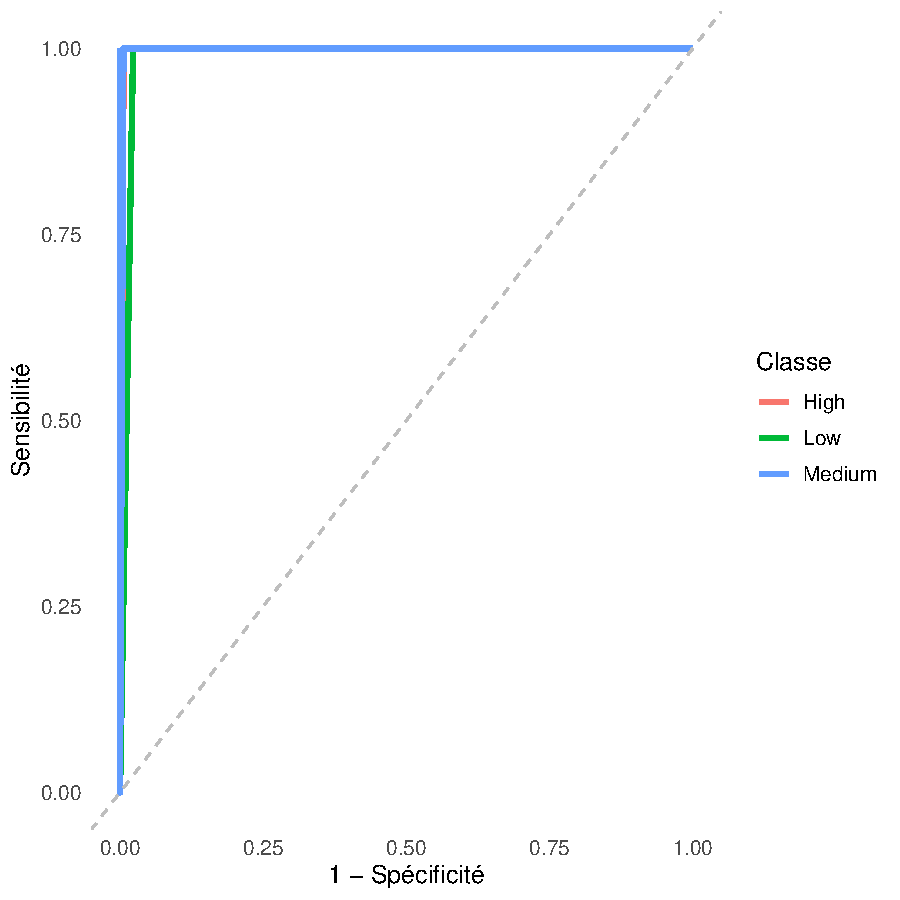
\includegraphics{dosfin-060}

\end{center}

\subsubsection{Matrice de confusion}

\begin{center}

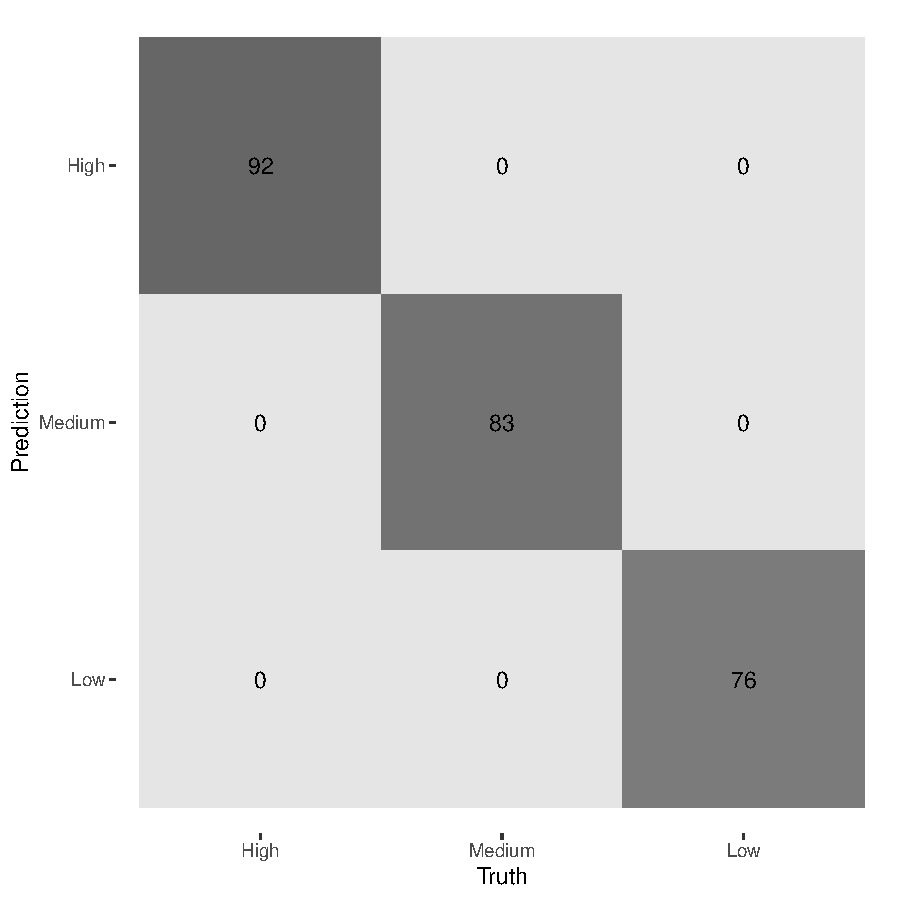
\includegraphics{dosfin-061}

\end{center}


\subsubsection{Importance des variables}

\begin{center}

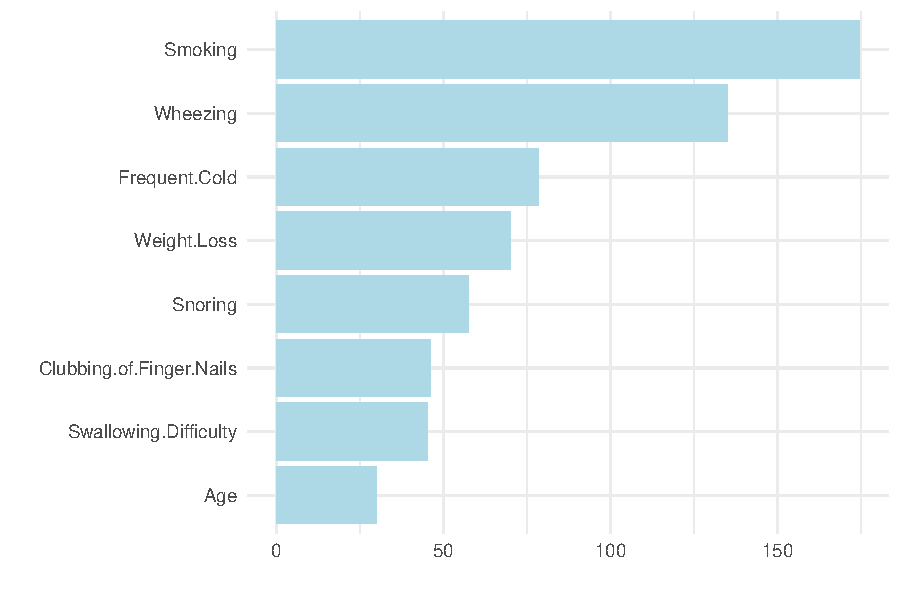
\includegraphics{dosfin-062}

\end{center}

\subsubsection{Interprétation}

Comme mentionné précédemment, ce modèle parvient à prédire parfaitement les données de test, ce qui témoigne de sa robustesse.  
Concernant l’importance des variables, aucune ne domine réellement, à l’exception de la variable \textit{smoking} qui ressort légèrement, sans pour autant être écrasante.  
Il s’agit à ce stade du modèle le plus performant et le plus prometteur.

\newpage

\subsection{Boosting}

Le modele XGBoost construit les arbres de maniere sequentielle, chaque nouvel arbre cherchant a corriger les erreurs des precedents.  
Cette approche permet une grande flexibilite et souvent de meilleures performances predictives, au prix d’un risque plus eleve de surapprentissage si elle est mal reglee.

Trois hyperparametres cles sont optimises :  
le nombre d'arbres construits (n\_trees),  
la profondeur maximale des arbres (tree\_depth),  
et le taux d'apprentissage (learning rate), qui controle l'impact de chaque nouvel arbre sur le modele global.

XGBoost est un modele puissant, capable de s'adapter a des structures complexes tout en conservant de bonnes capacites predictives sur des jeux de donnees varies.



\subsubsection{Optimisation des hyperparamêtres}



\begin{center}

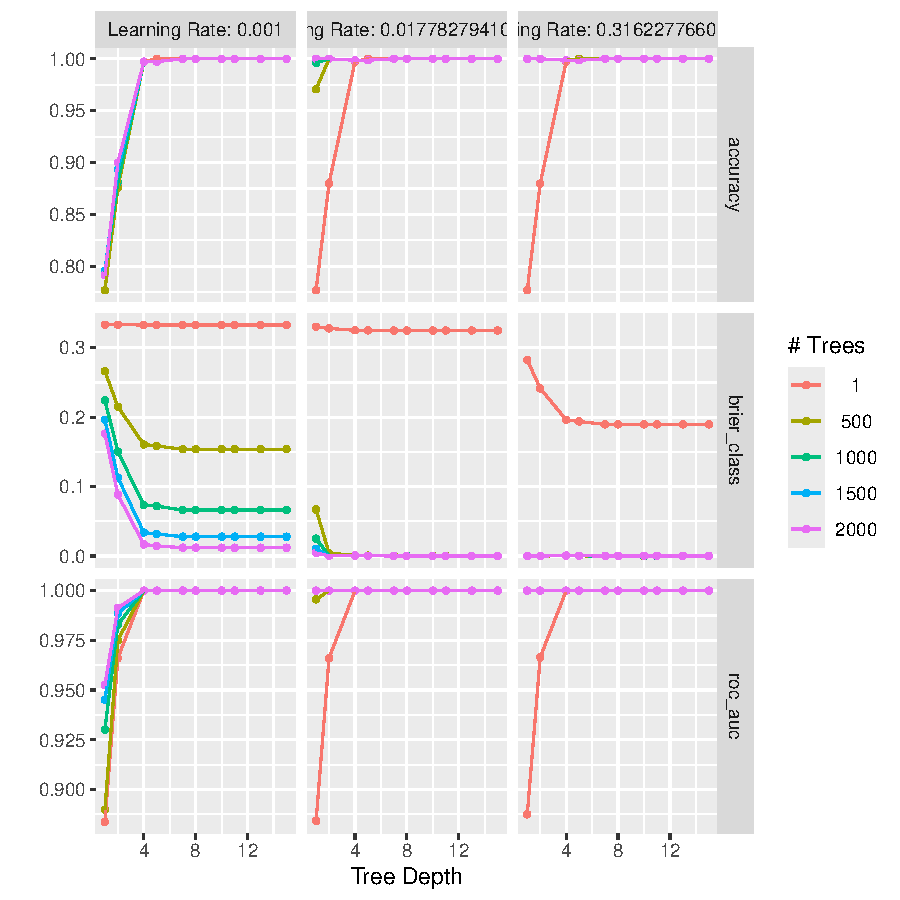
\includegraphics{dosfin-064}

\end{center}

Comme pour la foret aleatoire, plusieurs combinaisons d'hyperparametres permettent d'obtenir un score maximal. Nous choisissons ici un taux d'apprentissage de 0.0177828 avec 1500 arbres de profondeur 1.


\newpage

\subsubsection{Résultat sur le modèle}

\begin{center}


\begin{table}[ht]
\centering
\begin{tabular}{rllr}
  \hline
 & .metric & .estimator & .estimate \\ 
  \hline
1 & accuracy & multiclass & 100.00 \\ 
  2 & f\_meas & macro & 100.00 \\ 
  3 & recall & macro & 100.00 \\ 
  4 & precision & macro & 100.00 \\ 
  5 & spec & macro & 100.00 \\ 
  6 & roc\_auc & macro & 100.00 \\ 
  7 & error & macro & 0.00 \\ 
   \hline
\end{tabular}
\caption{Résultats} 
\end{table}


\end{center}

\subsubsection{Courbe ROC}

\begin{center}

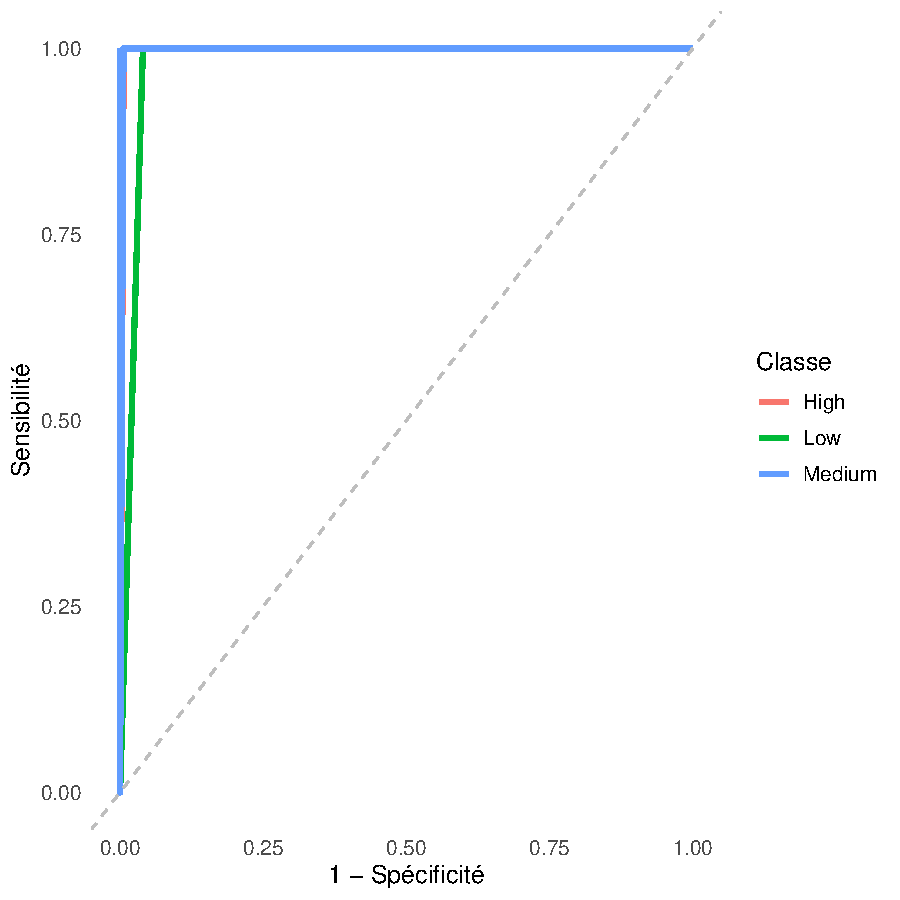
\includegraphics{dosfin-065}

\end{center}

\subsubsection{Matrice de confusion}

\begin{center}

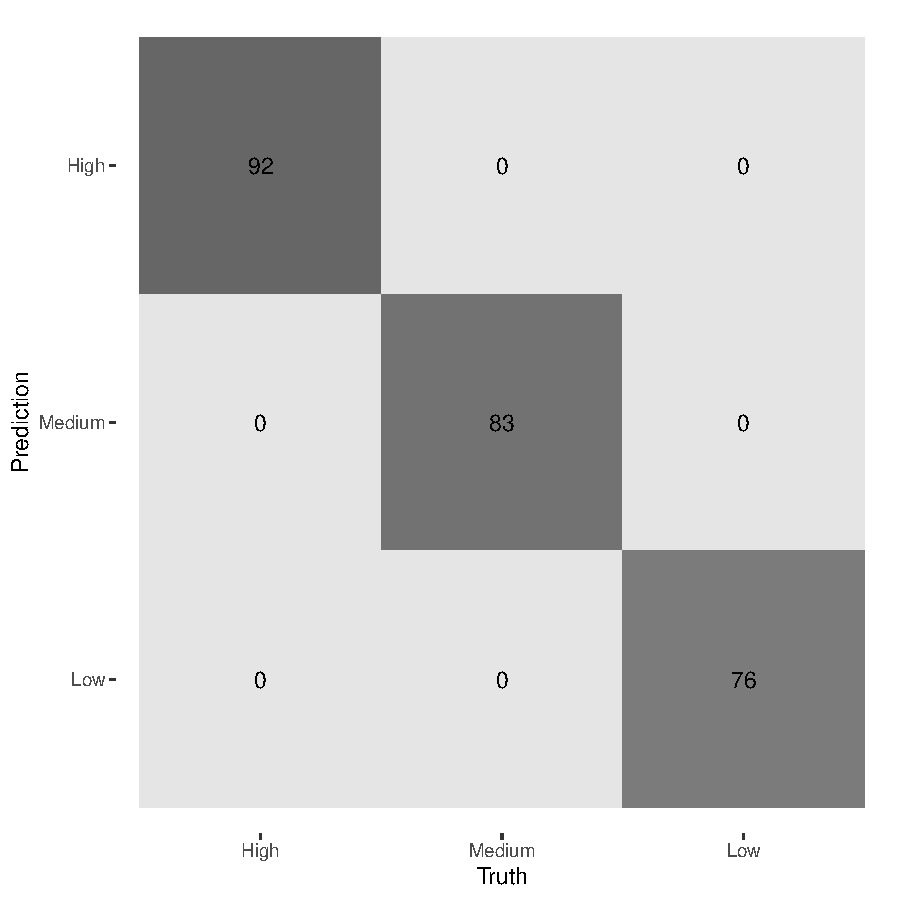
\includegraphics{dosfin-066}

\end{center}


\subsubsection{Importance des variables}

\begin{center}



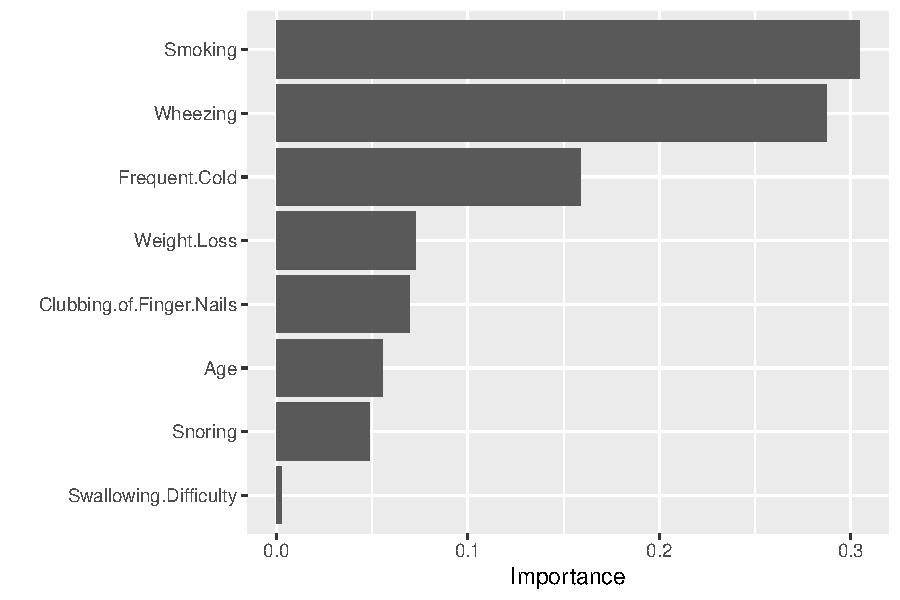
\includegraphics{dosfin-068}

\end{center}

\newpage

\subsubsection{Interprétation}

Nous constatons donc, comme pour la foret aleatoire, que les donnees test ont ete predites a la perfection.  
Ce modele se situe donc au meme niveau que la foret aleatoire en termes de performance.  
Cependant, nous observons une difference notable dans l'importance des variables : deux d'entre elles semblent dominer.  
Comme mentionne precedemment, ce modele est plus sensible au surapprentissage. Il se pourrait donc qu'il se soit trop appuye sur les specificites du jeu de donnees sans reellement bien generaliser.  
Nous discuterons du modele final choisi dans la section suivante.


\section{Modèle retenu}

\begin{center}
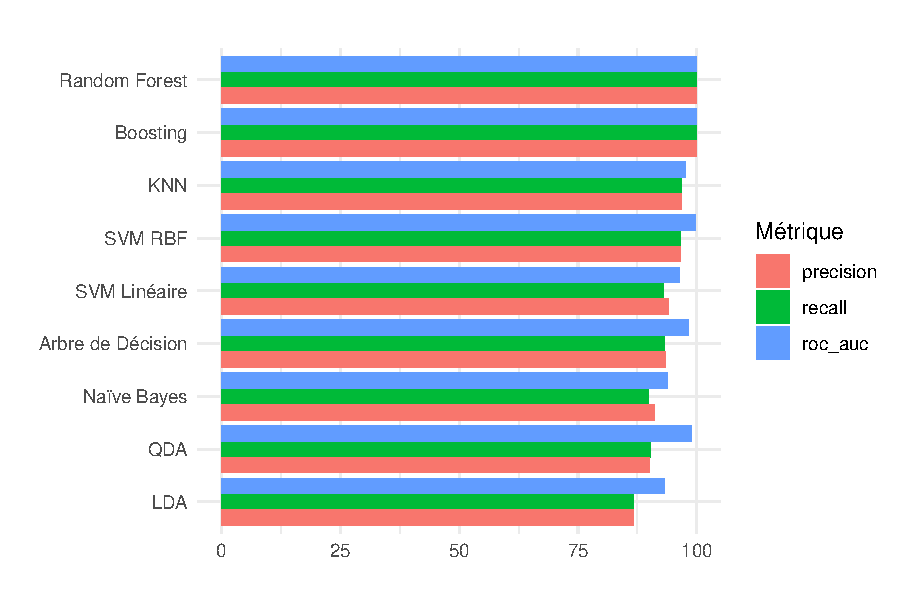
\includegraphics{dosfin-069}

\end{center}

Voici un petit recapitulatif des modeles les plus performants.  
Nous voyons bien que les modeles s'appuyant sur des hypotheses sur la distribution sont en moyenne les moins performants.  
De plus, notre jeu de donnees semble mal separer les classes de maniere lineaire.  
Enfin, nous constatons que deux modeles predisent parfaitement les donnees test : le boosting et la foret aleatoire.  
Nous retiendrons cette derniere, etant plus robuste face au surapprentissage que peut presenter le boosting, comme nous l'avons vu precedemment.  

Un cadre d'utilisation possible de ce modele serait des questionnaires de sensibilisation en ligne.  
Les individus pourraient y saisir leurs informations en fonction des variables utilisees afin d'obtenir une prediction de leur risque de developper un cancer du poumon.  
Cela permettrait de les sensibiliser aux risques de cette maladie et de les encourager a effectuer des tests de depistage.

\newpage

\section{Conclusion}

\end{document}
